\documentclass[xcolor=table, aspectratio=169,ignorenonframetext]{beamer}

%\documentclass{article}
%\usepackage{beamerarticle}

%\usepackage{arev}
\usepackage{amsmath,amssymb,amscd}
\usepackage{dsfont}
\usepackage{mathrsfs}
\usepackage{yfonts}
\usepackage{bm}
\usepackage{graphicx}
\usepackage{tabularx}
\usepackage{animate}
\usepackage{listings}
%\usepackage{ifthen}
\usepackage{pifont}

%\usepackage{xeCJK}
%\usepackage{fontspec}
%\newfontfamily\cjkfont{PingFang SC}
%\setCJKmainfont{PingFang SC}
\newcolumntype{x}{>{\centering\arraybackslash}X}
\renewcommand{\arraystretch}{1.5}
\DeclareMathOperator{\img}{img}
\DeclareMathOperator{\hhom}{Hom}
\newcommand{\uone}{\text U(1)}
\DeclareMathOperator{\id}{id}
\usepackage{tikz}
	\usetikzlibrary{calc}
	\usetikzlibrary{arrows,shapes, positioning, matrix}
	\usetikzlibrary{decorations.markings}
	\tikzstyle arrowstyle=[scale=1]
  \tikzstyle string=[thick,postaction={decorate,decoration={markings,
      mark=at position .55 with {\arrow[arrowstyle]{stealth}}}}]

\usepackage{tikz-cd}
\usepackage{pgffor}
\newcommand{\cohosub}[1]{\scalebox{0.72}{\textswab{#1}}}
\newcommand{\cohosubsub}[1]{\scalebox{0.6}{\textswab{#1}}}
\newcommand{\coho}[1]{\textswab{#1}}


\mode<presentation>
{
  %\usetheme{Warsaw}
  % or ...
  %\useoutertheme{rectangle}
  \setbeamertemplate{frametitle}[default][center]
  \defbeamertemplate{itemize item}{flat}{\begin{pgfpicture}{-1ex}{0ex}{1ex}{2ex}
      \pgfpathcircle{\pgfpoint{0pt}{.6ex}}{0.6ex}
      \pgfusepath{fill}
    \end{pgfpicture}%
  }
  \defbeamertemplate{itemize subitem}{flat}{\footnotesize\raise0.5pt\hbox{\textbullet}}
  \defbeamertemplate{itemize subsubitem}{flat}{\footnotesize\raise0.5pt\hbox{\textbullet}}

  %\useinnertheme{circles}
  \setbeamertemplate{items}[flat]
  \setbeamertemplate{sections/subsections in toc}[circle]
  \setbeamertemplate{blocks}[rounded]
  \setbeamertemplate{title page}[default][colsep=-4bp,rounded=true]
  \setbeamertemplate{part page}[default][colsep=-4bp,rounded=true]
  \setbeamercovered{transparent}
  %\usecolortheme{spruce}
  %\definecolor{THU}{RGB}{116,61,130}
  \definecolor{mbg}{RGB}{0,0,160}
  \setbeamercolor*{palette primary}{fg=white,bg=mbg}
  \setbeamercolor*{titlelike}{parent=palette primary}
  \setbeamercolor*{structure}{fg=mbg}
  \setbeamercolor{frametitle}{fg=white,bg=mbg}
  % or whatever (possibly just delete it)
  \setbeamercolor{block title}{bg=mbg,fg=white}
  \setbeamercolor{block body}{bg=mbg!15}


  \addtobeamertemplate{navigation symbols}{}{ \hspace{1em}%
    \usebeamerfont{footline}%
    \insertframenumber / \inserttotalframenumber }
}


%\usepackage[english]{babel}
% or whatever

%\usepackage[latin1]{inputenc}
% or whatever

%\usepackage{times}
%\usepackage[T1]{fontenc}
% Or whatever. Note that the encoding and the font should match. If T1
% does not look nice, try deleting the line with the fontenc.

\title % (optional, use only with long paper titles)
{Computing the classification of symmetry-protected topological phases with homological algebra}
\author[Y Qi] % (optional, use only with lots of authors)
{Yang~Qi}
% - Give the names in the same order as the appear in the paper.
% - Use the \inst{?} command only if the authors have different
%   affiliation.

\institute[Fudan] % (optional, but mostly needed)
{
Department of Physics, Fudan University.
}
% - Use the \inst command only if there are several affiliations.
% - Keep it simple, no one is interested in your street address.

%\date{2016 Annual Meeting of Fudan CFTPP} % (optional, should be abbreviation of conference name)
%{Fudan University, Oct 13 2015}
\date{Oct. 17th, 2020}
% - Either use conference name or its abbreviation.
% - Not really informative to the audience, more for people (including
%   yourself) who are reading the slides online

%\subject{Theoretical Physics}
% This is only inserted into the PDF information catalog. Can be left
% out.



% If you have a file called "university-logo-filename.xxx", where xxx
% is a graphic format that can be processed by latex or pdflatex,
% resp., then you can add a logo as follows:

\pgfdeclareimage[height=1cm]{university-logo}{../resources/fudan}
\logo{\pgfuseimage{university-logo}}



% Delete this, if you do not want the table of contents to pop up at
% the beginning of each subsection:
\AtBeginSection[]
{
  \begin{frame}<beamer>{Outline}
			\tableofcontents[currentsection,currentsubsection]
  \end{frame}
}
%\AtBeginSubsection[]
%{
 % \begin{frame}<beamer>{Outline}
  %  \tableofcontents[currentsection,currentsubsection]
  %\end{frame}
%}


\begin{document}

\begin{frame}
  \titlepage
\end{frame}

\begin{frame}{References}
\begin{itemize}
\item Zhi-Da Song: Princeton University.
\item Chen Fang: Institute of Physics, Beijing.
\item Yunqing Ouyang: Fudan University.
\item Qing-Rui Wang: Yale University.
\item Zheng-Cheng Gu: Chinese University of Hong Kong.
\begin{center}
	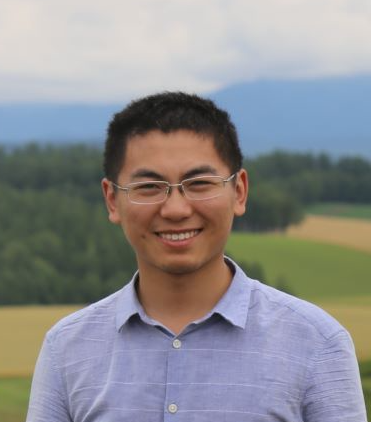
\includegraphics[height=2cm]{../people/zhidasong}
	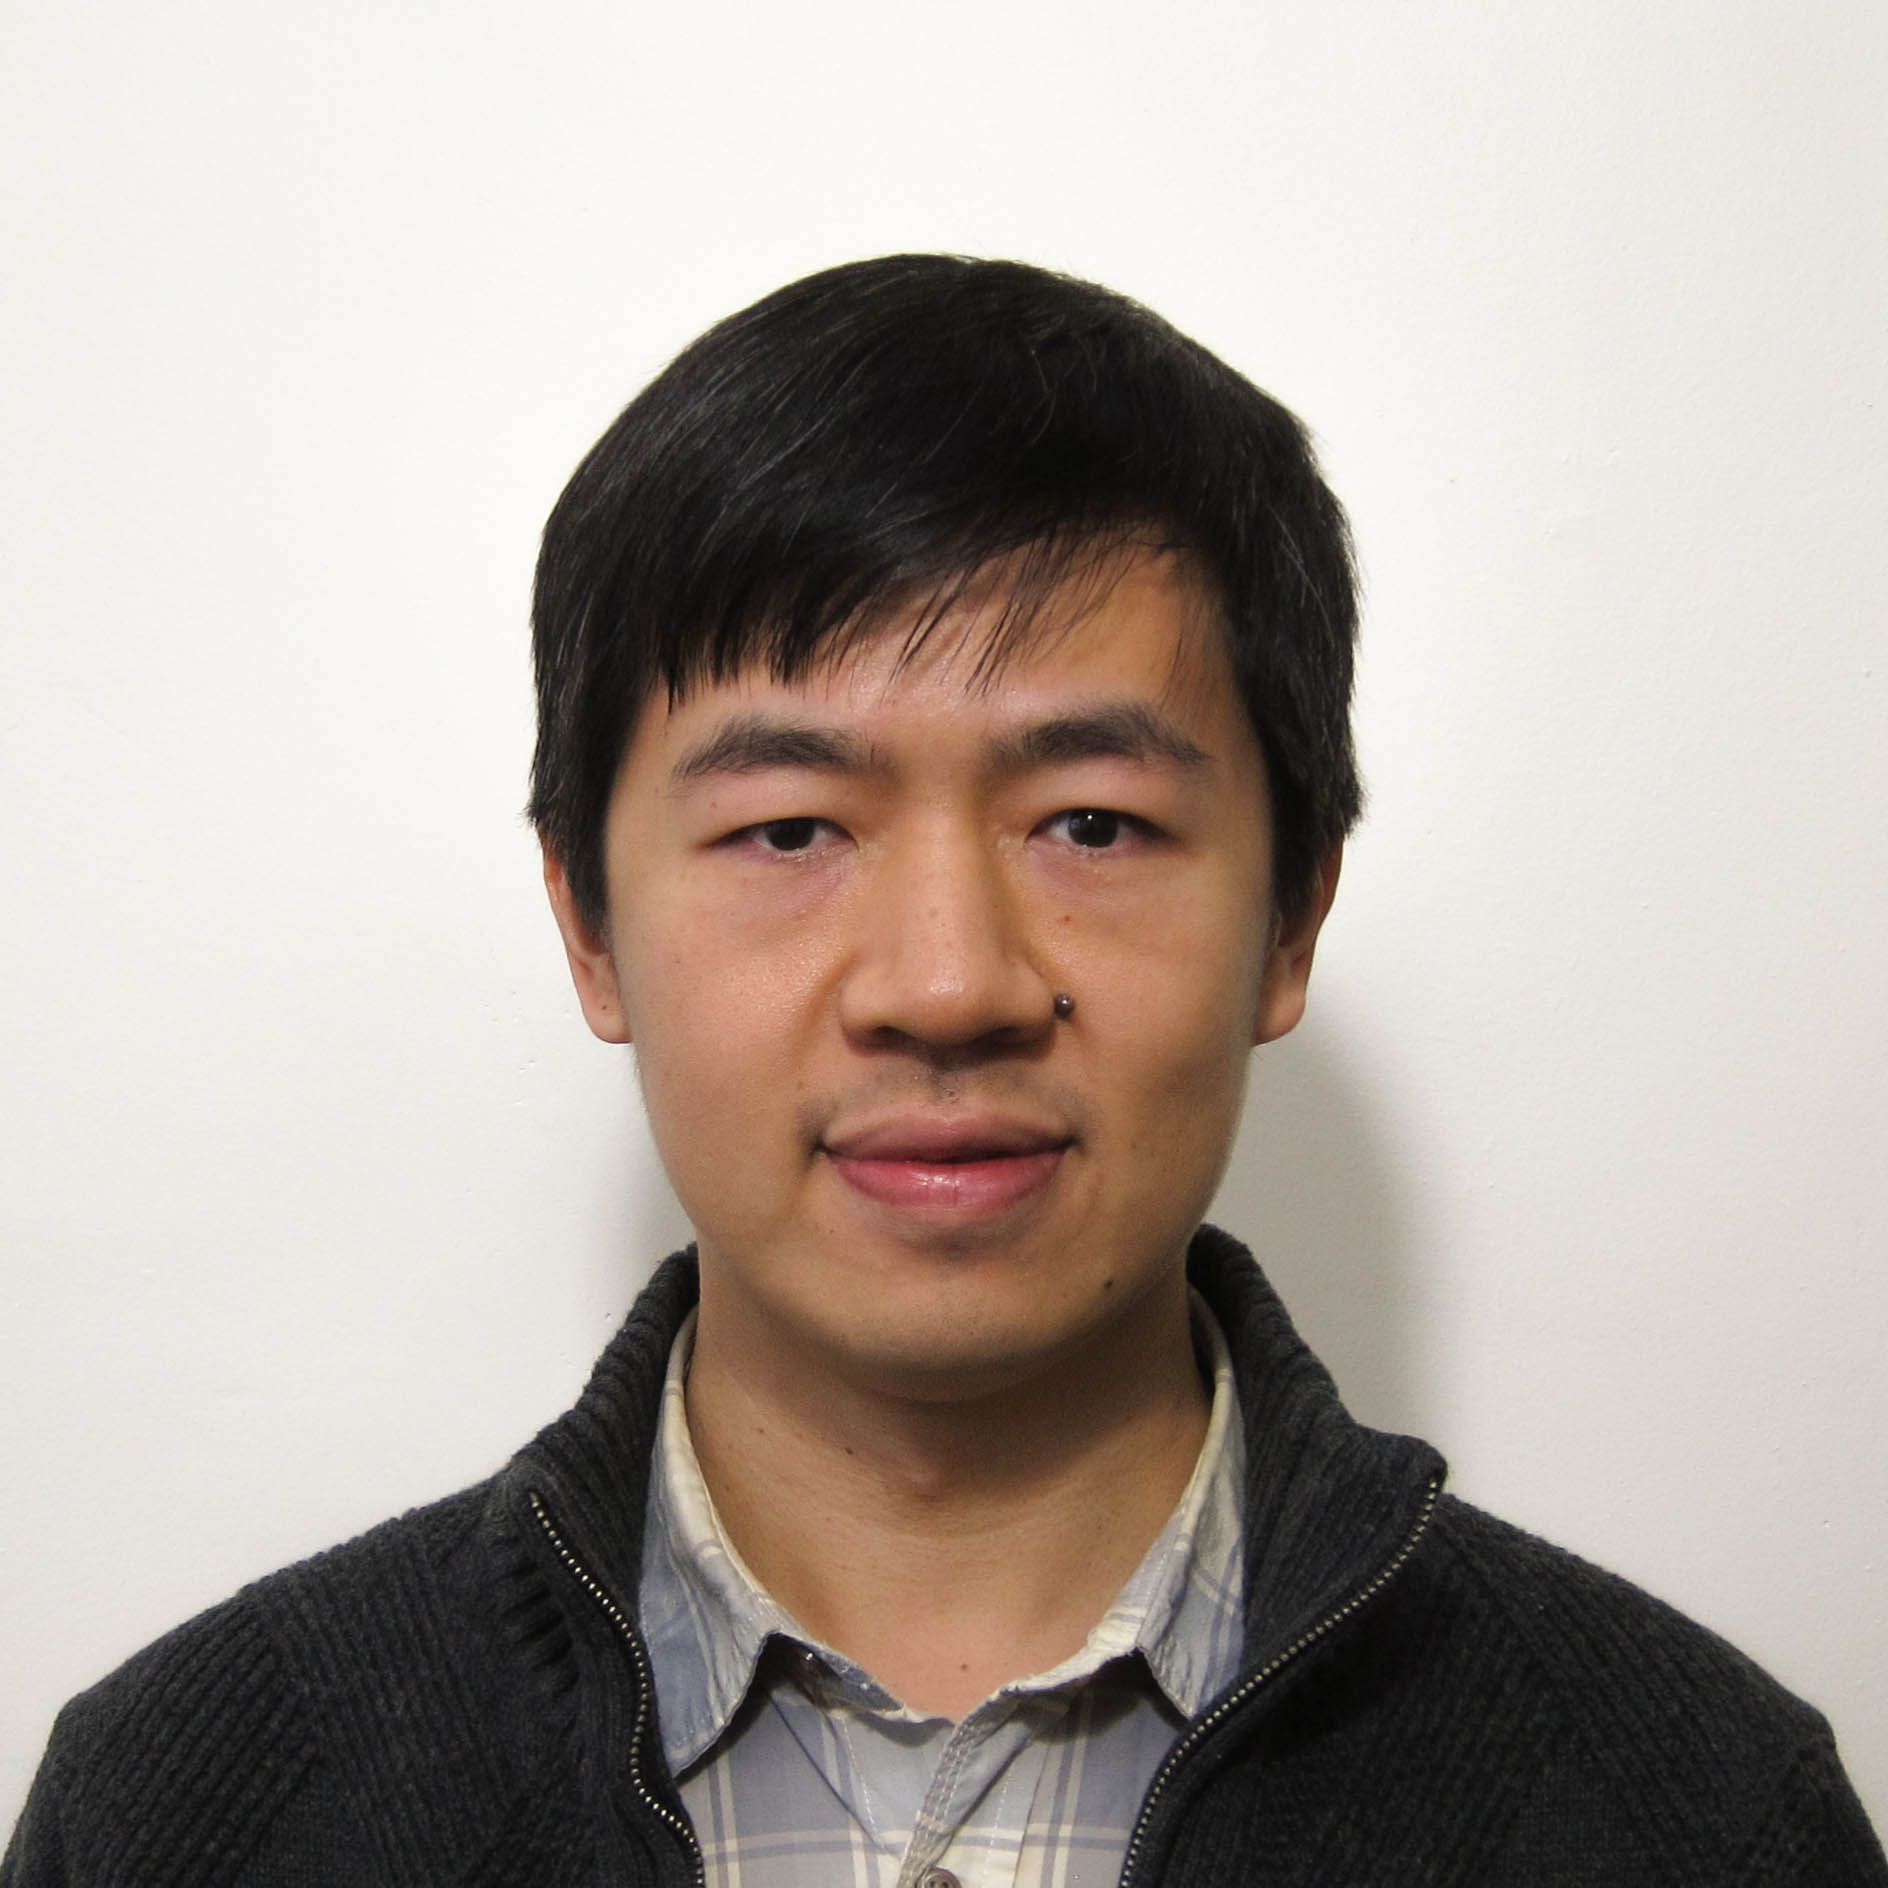
\includegraphics[height=2cm]{../people/chenfang}
        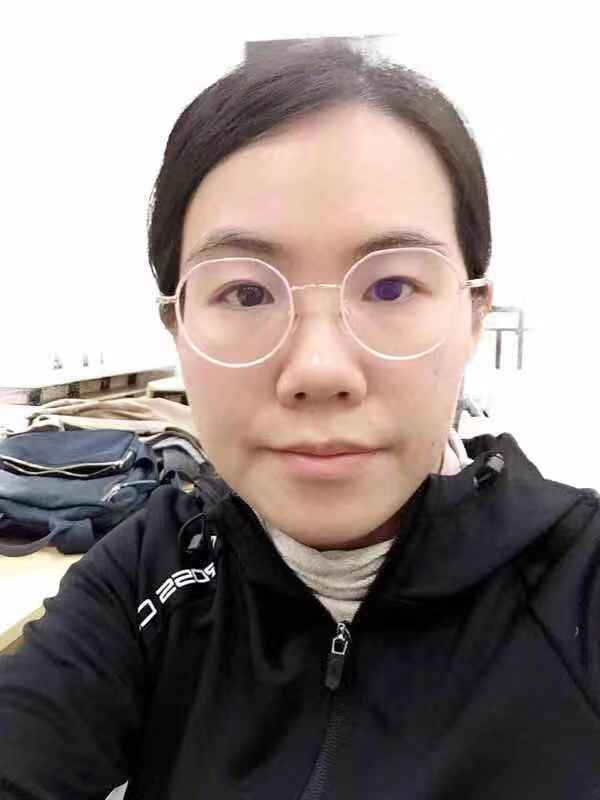
\includegraphics[height=2cm]{../people/yunqing}
        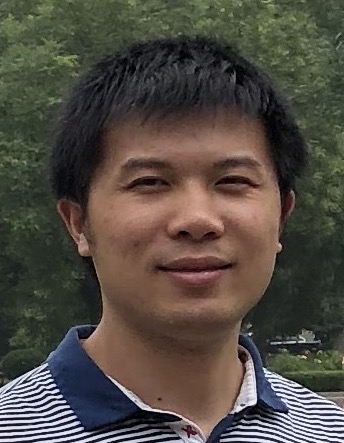
\includegraphics[height=2cm]{../people/qingrui}
        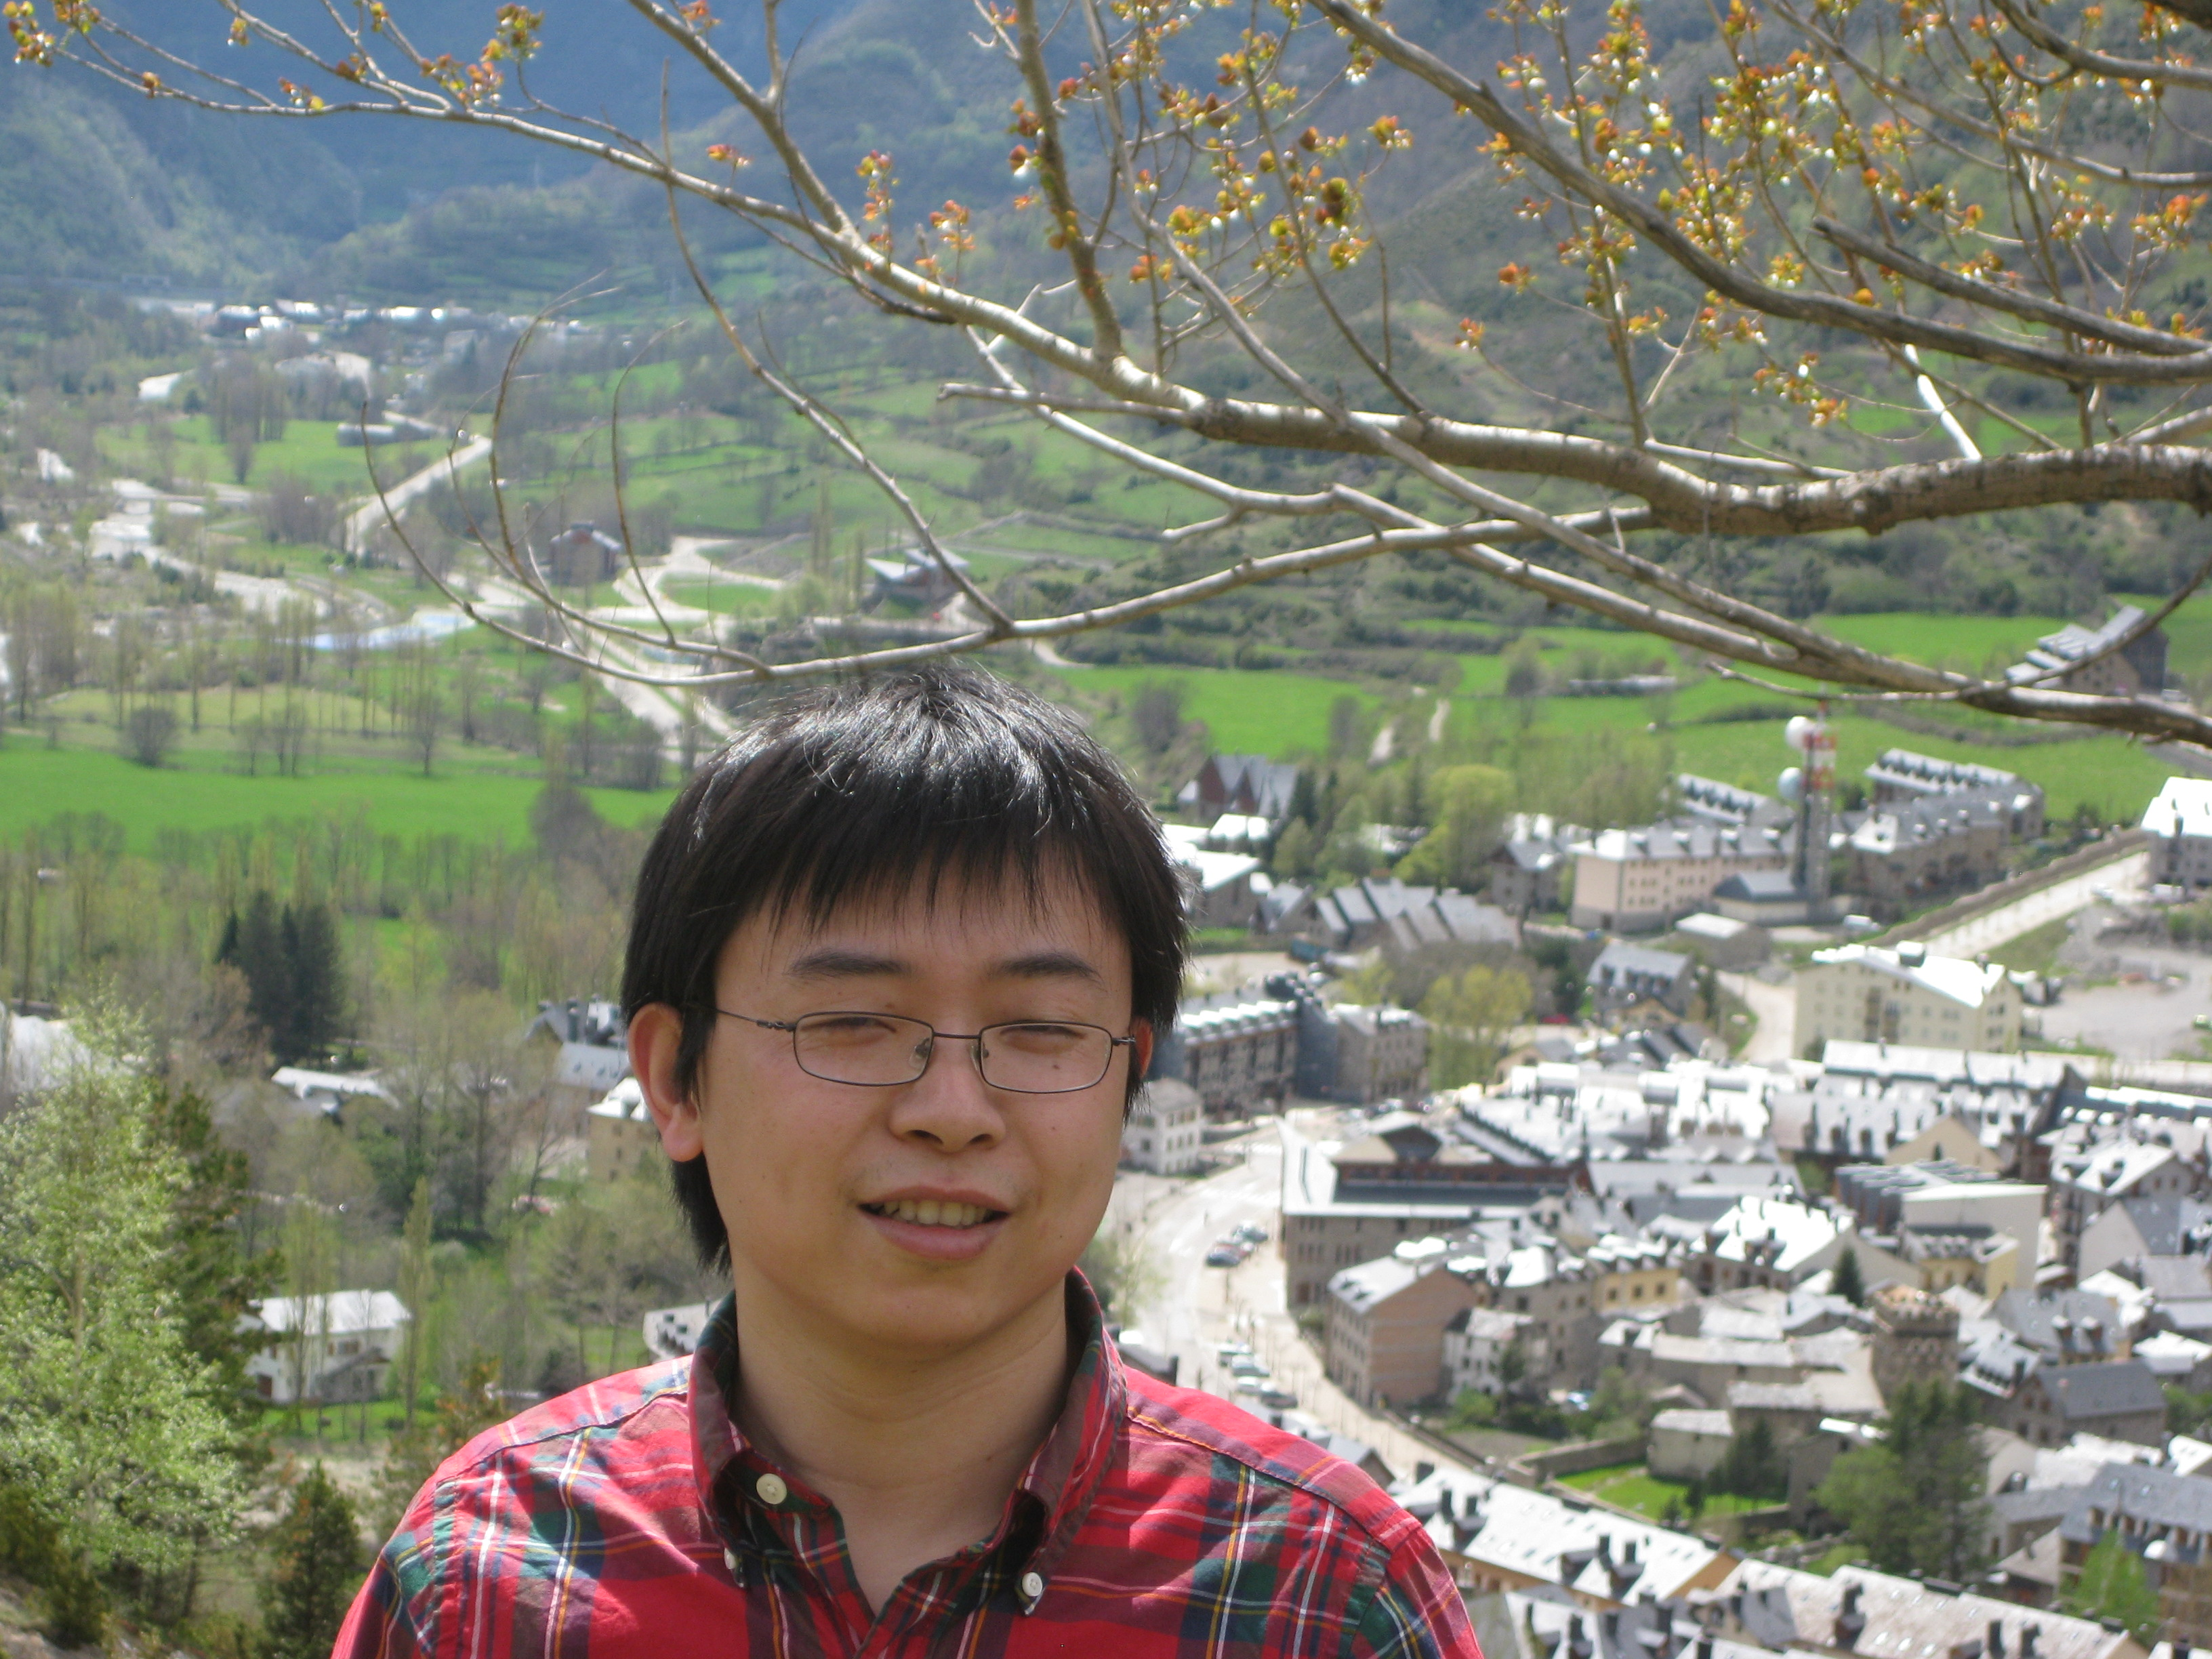
\includegraphics[height=2cm]{../people/zhengcheng}
\end{center}
\item Zhida Song, Chen Fang and Yang Qi, Nature Communications \textbf{11}, 4197 (2020).
\item Yunqing Ouyang, Qing-Rui Wang, Zheng-Cheng Gu and Yang Qi, arXiv:2005.06572.
\end{itemize}
\end{frame}

\begin{frame}{Outline}
	%\begin{columns}
	%\column{.7\textwidth}
		\tableofcontents
  %\end{columns}
  % You might wish to add the option [pausesections]
\end{frame}

\section{Introduction to SPT states}

\begin{frame}{Landau's paradigm: symmetry breaking}
  Traditional phases are organized in Landau's paradigm.
  \begin{enumerate}
  \item Crystal: breaking translation symmetry.
  \item Magnet: breaking spin-rotation symmetry.
  \item Superconductor: breaking U(1) charge-conservation symmetry.
  \end{enumerate}
  \begin{center}
    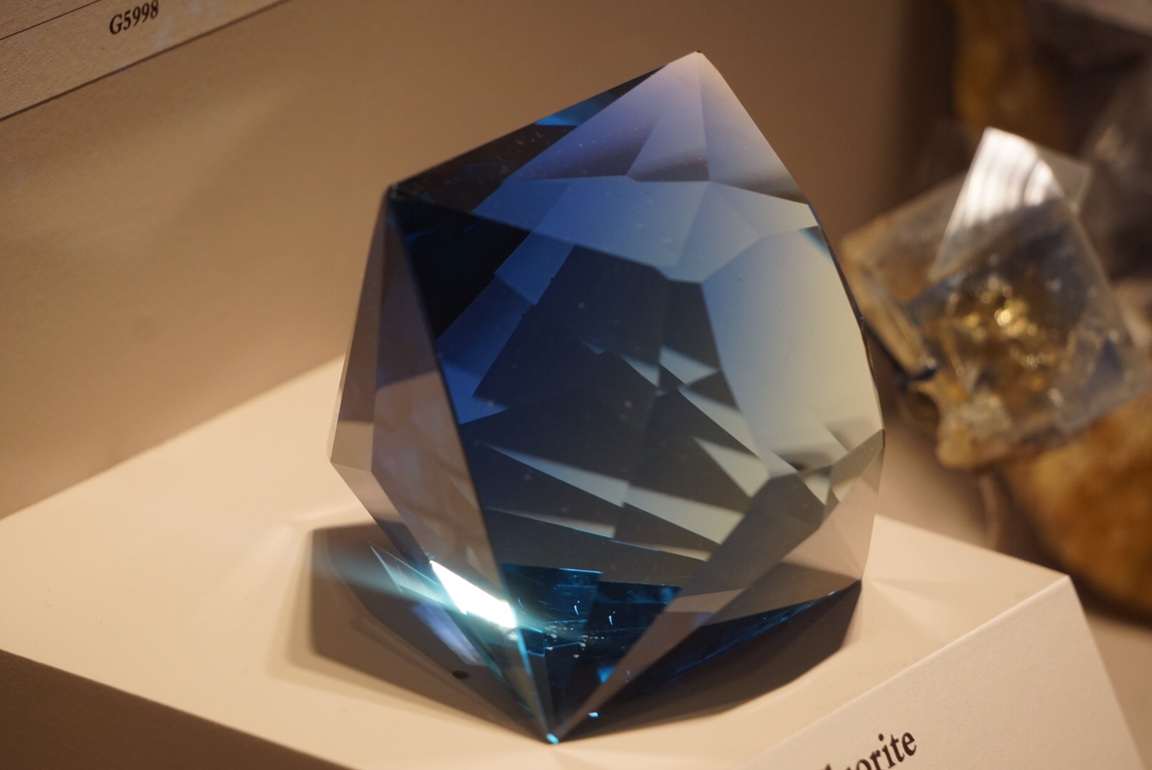
\includegraphics[height=2.5cm]{../resources/crystal}~~
    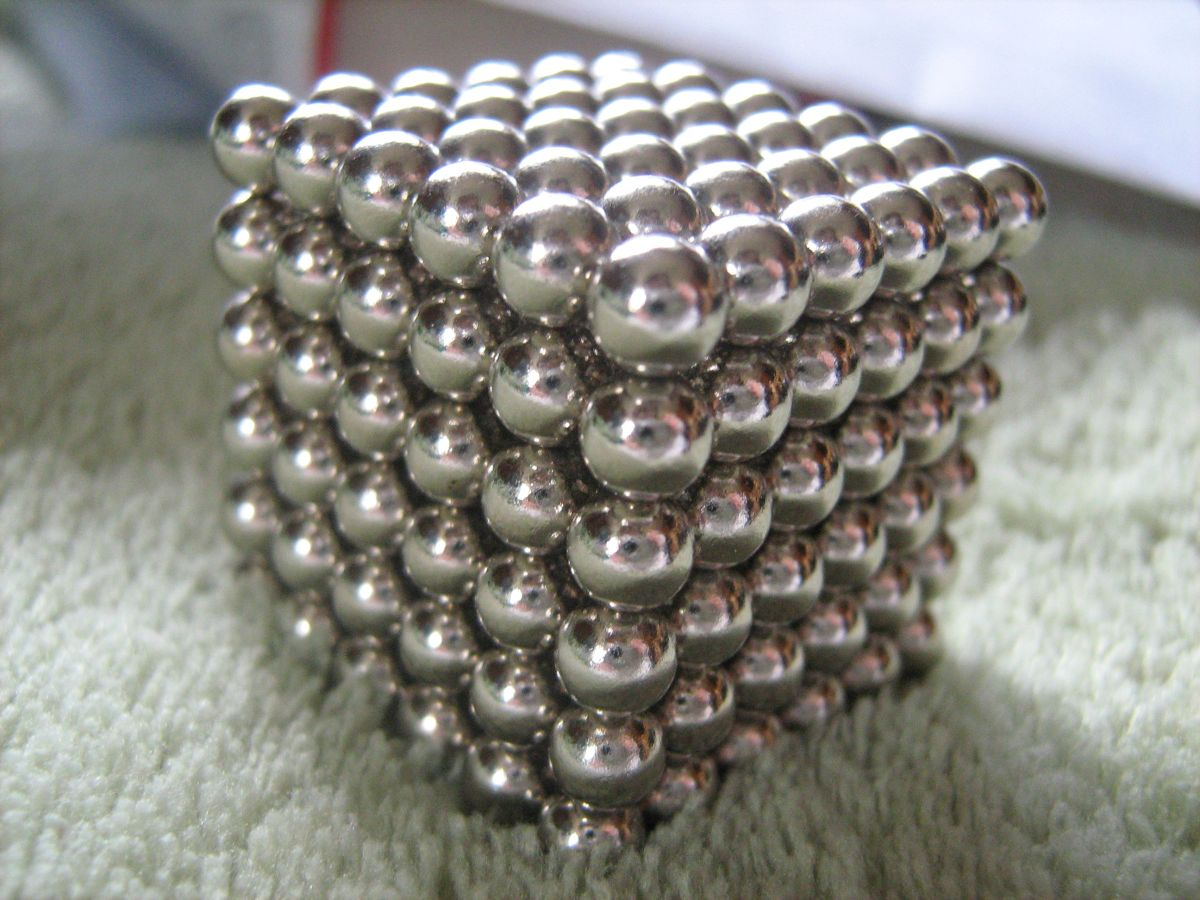
\includegraphics[height=2.5cm]{../resources/magnet}~~
    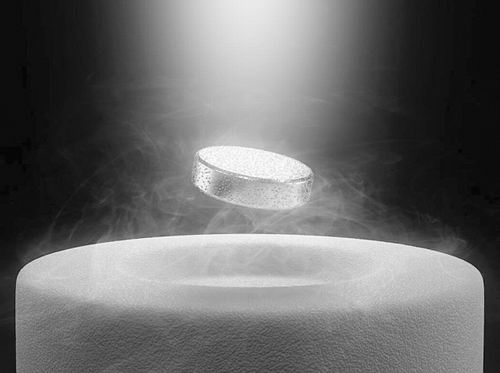
\includegraphics[height=2.5cm]{../resources/sc}
  \end{center}
\end{frame}

\begin{frame}
  \frametitle{Symmetry-Protected Topological (SPT) states}
\begin{itemize}
\item SPT: gapped topological phases beyond Landau paradiam.
\item Cannot be smoothly connected to a trivial state without closing gap or breaking symmetry.
\item Symmetry-protected gapless surface states.
%\item Free-fermion states: topological insulators, topological superconductors.
%\item Bosonic SPTs: Haldane chain, CZX/Levin-Gu state, etc.\\
%\emph{Xie Chen, Zheng-Cheng Gu, Zheng-Xin Liu and Xiao-Gang Wen, Science 2012.}
%\item Interacting fermionic SPTs.
\end{itemize}
\begin{center}
		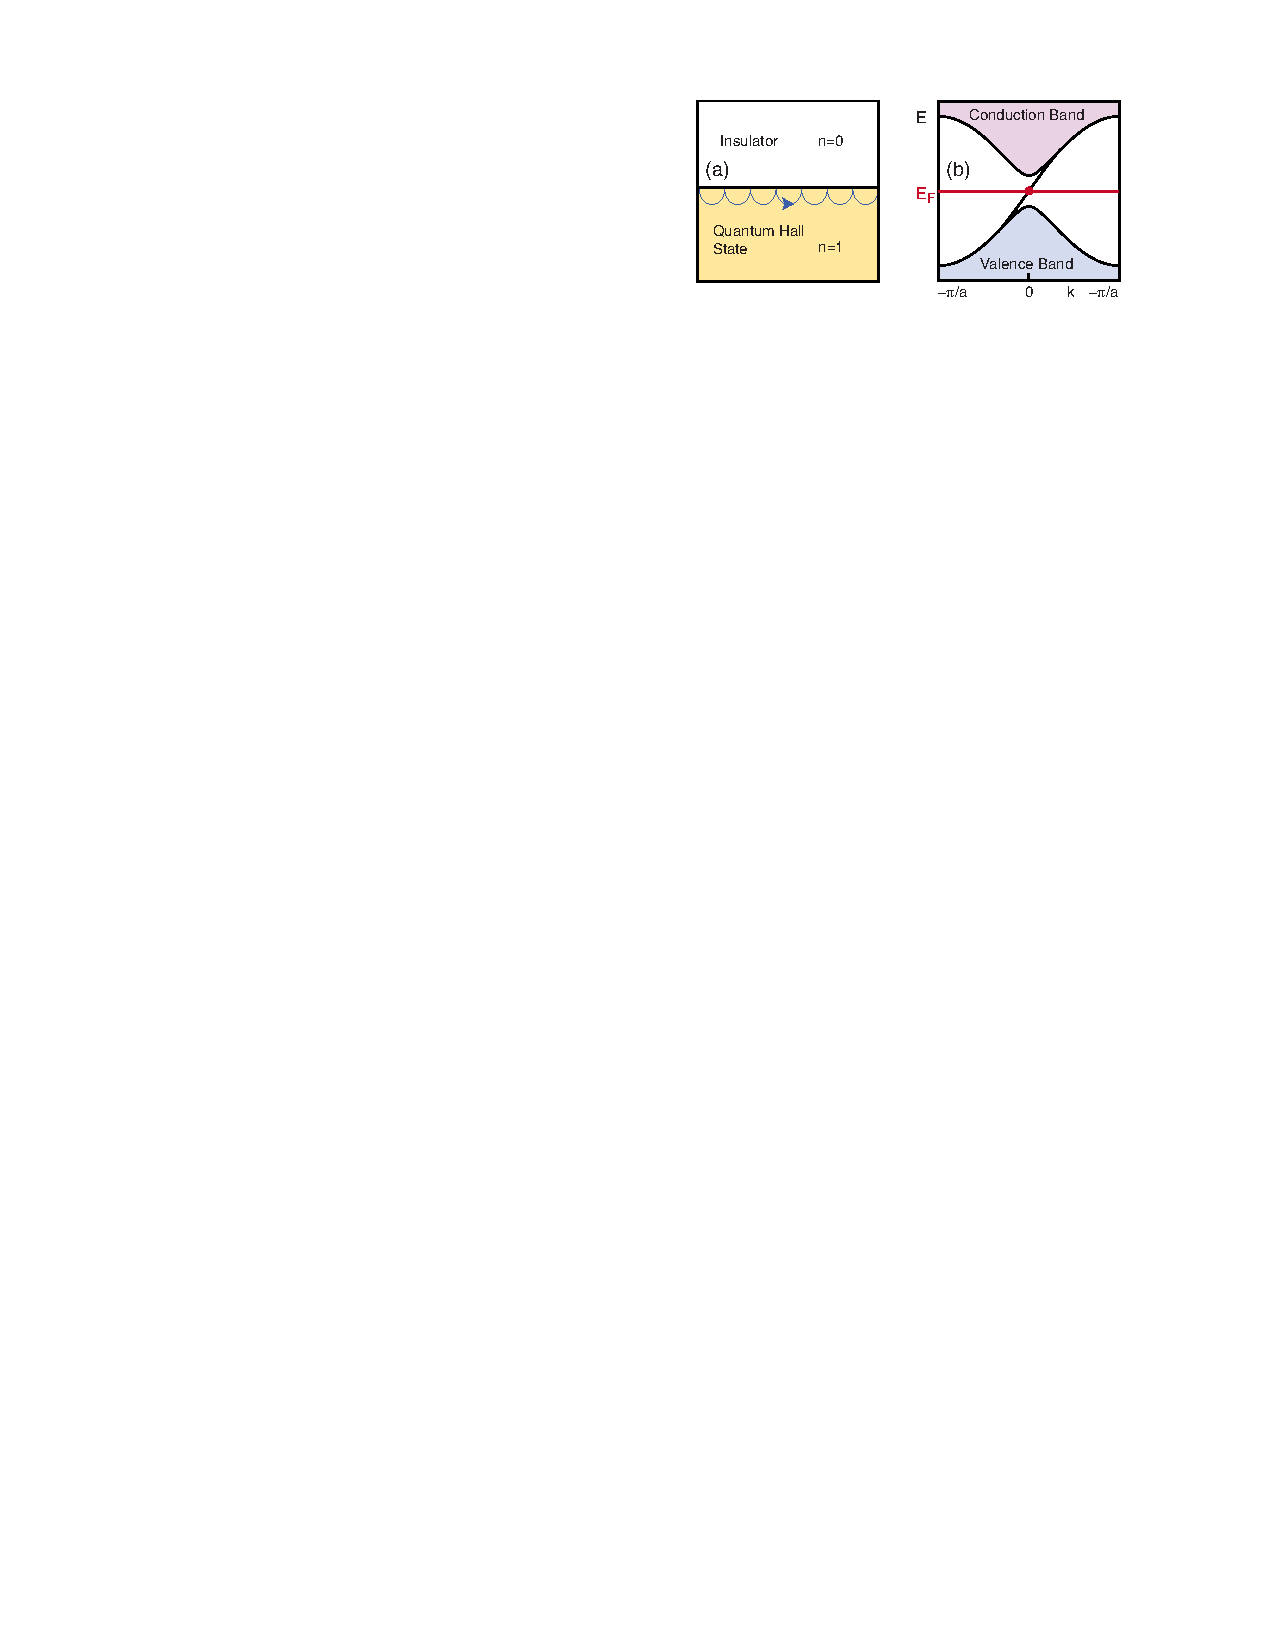
\includegraphics[width=8cm]{../spspt/qhe_edge}
\end{center}
\end{frame}

\begin{frame}
  \frametitle{Laughlin's argument}
  \begin{block}{How to detect an SPT state?}
    Bulk is trivial locally, and edge is too complicated.
  \end{block}
  Laughlin's argument on integer quantum hall / Chern insulators.
  \begin{itemize}
  \item Threading a magnetic flux ($\Phi_0 = hc/e$) through the hole of a cylinder.
  \item $\Phi(t)\Rightarrow E_y\Rightarrow I_x$.
  \item $ne$-charge is transported across the system.
  \item Hall conductance $\sigma_H$ is quantized.    
  \end{itemize}
  \begin{center}
    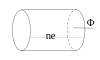
\includegraphics[scale=.5]{../spt-lecture/laughlin}    
  \end{center}
\end{frame}

\begin{frame}
	\frametitle{Generalizing a magnetic flux to a symmetry flux}
	\begin{itemize}
		\item Considier a finite, unitary symmetry group $G$.
		\item We can add a symmetry flux along a noncontractible loop $L$: after going around $L$, the Hilbert spaces are matched only after a symmetry operation $g$.
		\begin{center}
			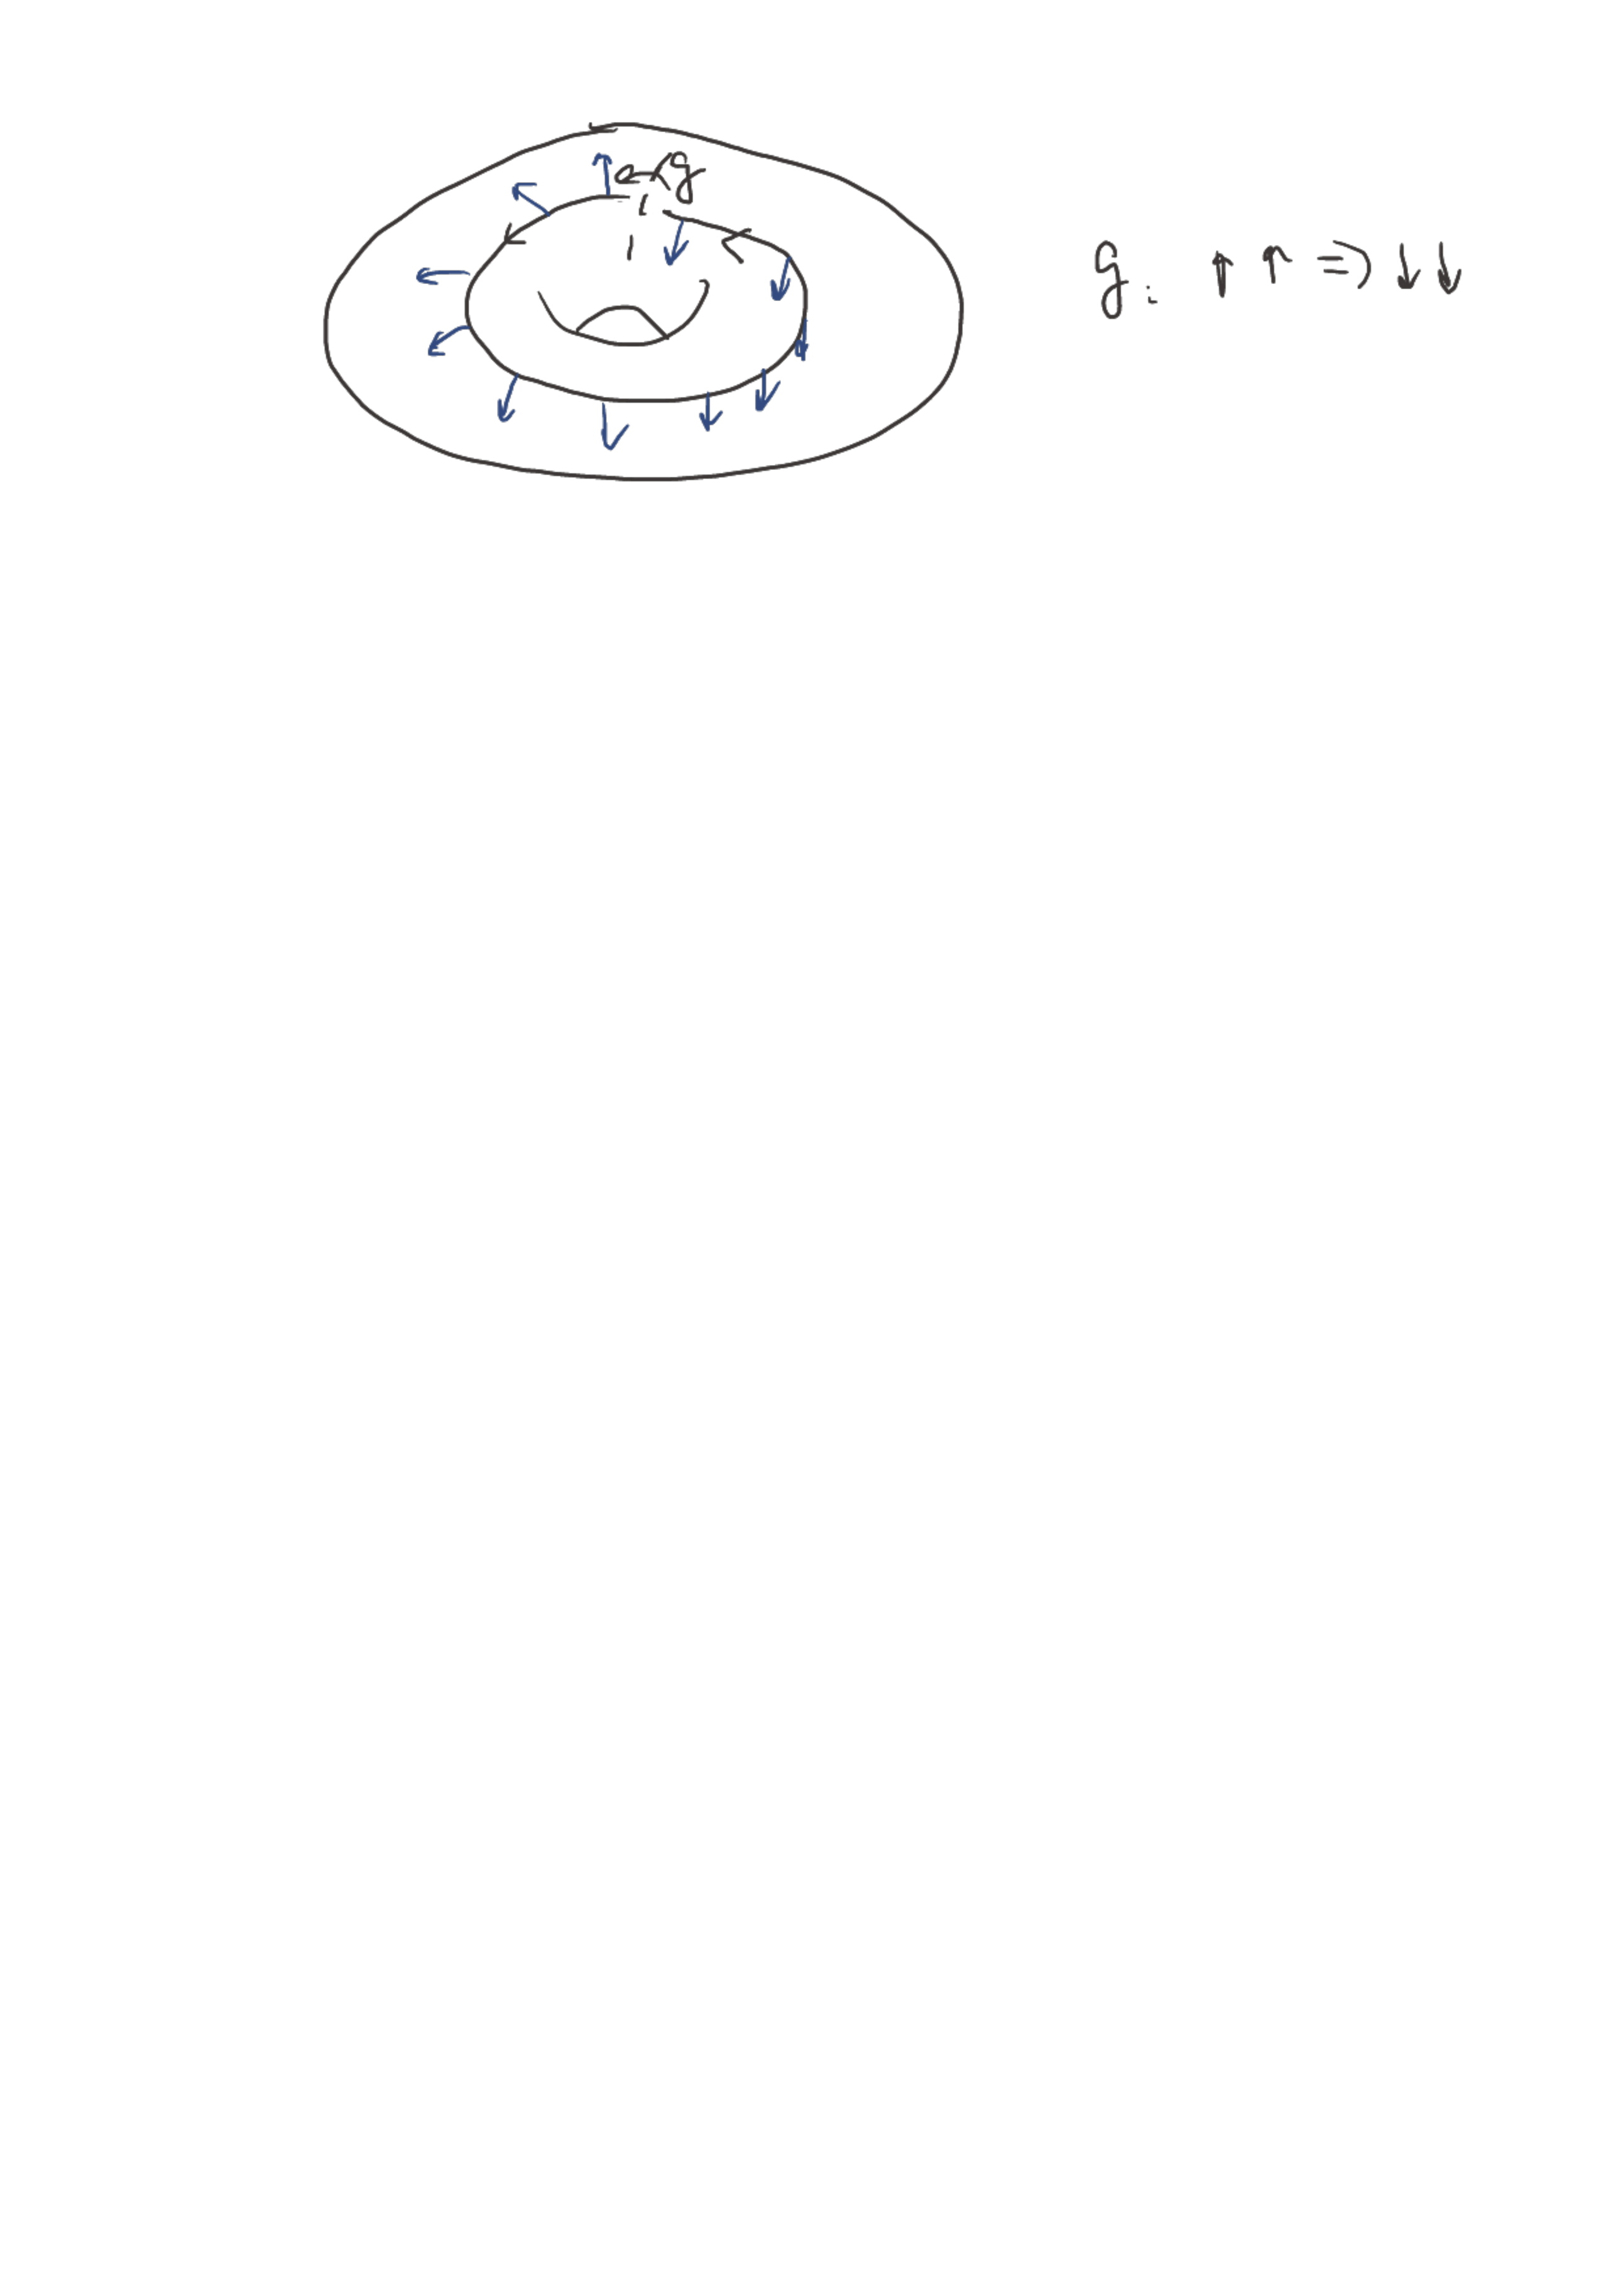
\includegraphics[height=3cm]{g-bundle}
		\end{center}
	\end{itemize}
\end{frame}

\begin{frame}
	\frametitle{Partition function of SPT state}
	\begin{itemize}
		\item Take a $(d+1)$-dimensional space-time manifold $M$,
		\item And $\gamma:\pi_1(M)\rightarrow G$, $M$ and $\gamma$ determines a $G$-bundle.
		\item An SPT phase: a partition function $Z(M,\gamma)$.
	\end{itemize}
	\begin{center}
		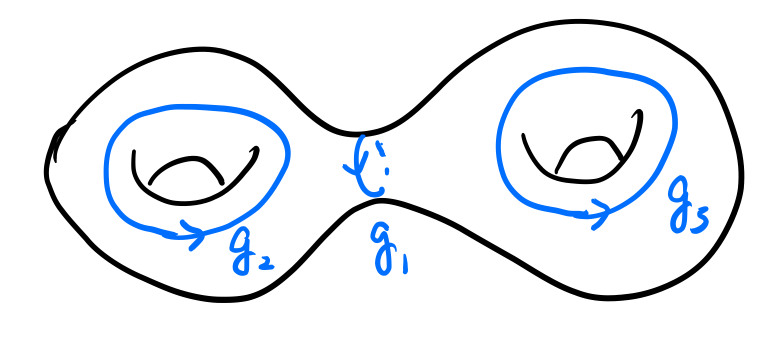
\includegraphics[height=3cm]{../spt-lecture/manifold}
	\end{center}
	{\small Dijkgraaf and Witten, Comm. Math. Phys. \textbf{129} 393 (1990).}
\end{frame}

\begin{frame}
	\frametitle{Universal bundle}
	\begin{itemize}
		\item Universal bundle: $p: EG \rightarrow BG$.
		\item Classifying space: $BG$ satisfying\\
		$\pi_1(BG) = G$, $\pi_2(BG)=0$, $\pi_3(BG)=0$, ...
		\item $\gamma:\pi_1(M)\rightarrow G=\pi_1(BG)$ can be extended to $\gamma:M\rightarrow BG$.
		\item Take a cocycle $\alpha\in H^{d+1}[BG, \uone]=H^{d+1}[BG, \mathbb R/\mathbb Z]$.
		\item We can construct $Z$:
		\[Z = \langle\gamma^\ast\alpha, [M]\rangle.\]
		$[M]$ is the fundamental class of $M$.
		\item $d$-dimensional bosonic SPT states are (partically) classified by $H^{d+1}[BG, \uone]=H^{d+1}[G, \uone]$.\\
		\emph{\small Xie Chen, Zheng-Cheng Gu, Zheng-Xin Liu and Xiao-Gang Wen, Science 2012.}
	\end{itemize}
\end{frame}

\begin{frame}
	\frametitle{Cohomology classes on $BG$ and inhomogeneous cocycle}
	\begin{itemize}
		\item Standard construction: $BG$ as a simplicial complex.
		\item All cells are simplices, $[g_1|g_2|\cdots|g_n]$.
		\item Boundary map:
		\[\partial[g_1|\cdots|g_n]=g_1[g_2|\cdots|g_n]
		-[g_1g_2|\cdots|g_n]+[g_1|g_2g_3|\cdots|g_n]-\cdots.\]
		\item This gives the inhomogeneous cocycle:
		$\alpha([g_1|\cdots|g_n])=\alpha(g_1,\ldots,g_n)$.
		\item This corresponds to the standard construction of $BG$.
	\end{itemize}
\begin{center}
	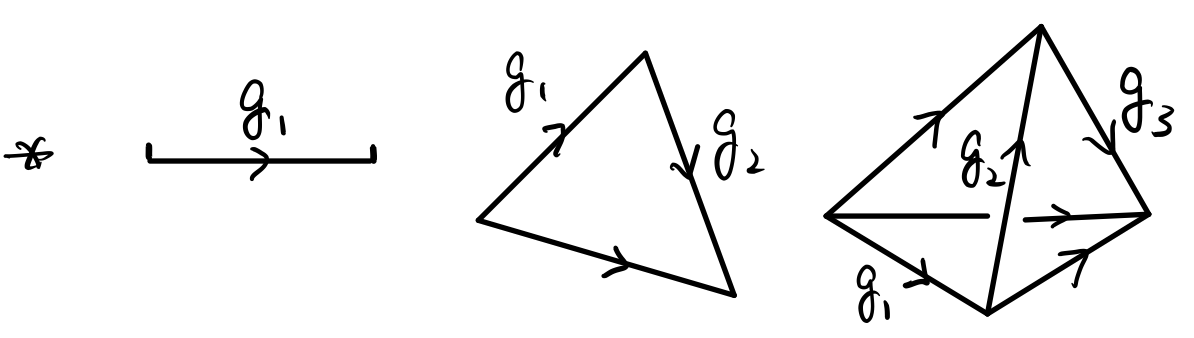
\includegraphics[width=10cm]{../chainmap/bg-std}
\end{center}
\end{frame}

\begin{frame}
	\frametitle{SPT phases are classified by generalized cohomology theories}
	\begin{itemize}
		\item D Gaiotto \& T Johnson-Freyd, JHEP \textbf{2019}, 7 (2019).
		\item Free-fermion SPT phases: K theory.
		\item (Interacting) bosonic SPT phases: $H^{d+1}[G, \uone_T]$.
		\item Interacting-fermion SPT phases: spin cobordism, etc.
                  $H^*[BG_b, ??]$.\\
                  Formula for the most general cases is still unknown:
                  \[1\rightarrow\mathbb Z_2^f\rightarrow G_f\rightarrow G_b\rightarrow1.\]
	\end{itemize}
\end{frame}

%\begin{frame}
%	\frametitle{Comparing construction and detection}
%	\begin{itemize}
%		\item Claim:
%		\[H^n[G, \uone] = H^n[BG, \uone] = H^n_G[EG, \uone].\]
%		\item Homotopy type of $BG$ is determined by $G$. $H^n[G, \uone]$ are invariants of $G$.
%		\item $d$-dimensional bosonic SPT phases are classified by
%		$H^{d+1}[G, \uone]$.
%		\item Lie-group symmetries?
%		\item Beyond-group-cohomology phases?
%	\end{itemize}
%\end{frame}

\section{Spectral sequence and real-space construction}

\begin{frame}
\frametitle{Space-group SPT}
\begin{itemize}
\item We consider $G/G_0 = SG$.
\item Thorngren and Else (2018): the classification is also given by group cohomology
\[H^{d+1}[G, \uone_{PT}].\]
\item Dimensional reduction: Liang Fu, Michael Hermele et al.\\
\emph{Examples: mirror SPT, weak SPT (translation symmetry).}
\item Patch construction: Zhida Song, Shengjie Huang, Yang Qi, Chen Fang and Michael Hermele, Sci. Adv. 2019.
\item A more general construction for bosonic SPTs.
\end{itemize}
\begin{center}
\begin{tikzpicture}[scale=.9]
\fill [blue!20] (0,0)--(1,1)--(1,3)--(0,2)--(0,0);
\draw (0,0)--(0,2)--(1,3);
\draw (-1.5,0)--(1.5,0)--(1.5,2)--(-1.5,2)--(-1.5,0);
\draw (1.5,0)--(2.5,1)--(2.5,3)--(1.5,2);
\draw (2.5,3)--(-.5,3)--(-1.5,2);
\end{tikzpicture}
\hspace{2em}
\begin{tikzpicture}[scale=.9]
\fill [blue!40,opacity=.5] (0,0)--(1,1)--(1,3)--(0,2)--(0,0);
\draw (0,0)--(0,2)--(1,3);
\fill [blue!40,opacity=.5] (.5,0)--(1.5,1)--(1.5,3)--(0.5,2)--(0.5,0);
\draw (.5,0)--(.5,2)--(1.5,3);
\fill [blue!40,opacity=.5] (1,0)--(2,1)--(2,3)--(1,2)--(1,0);
\draw (1,0)--(1,2)--(2,3);
\fill [blue!40,opacity=.5] (-.5,0)--(.5,1)--(.5,3)--(-0.5,2)--(-0.5,0);
\draw (-.5,0)--(-.5,2)--(.5,3);
\fill [blue!40,opacity=.5] (-1,0)--(0,1)--(0,3)--(-1,2)--(-1,0);
\draw (-1,0)--(-1,2)--(0,3);
\draw (-1.5,0)--(1.5,0)--(1.5,2)--(-1.5,2)--(-1.5,0);
\draw (1.5,0)--(2.5,1)--(2.5,3)--(1.5,2);
\draw (2.5,3)--(-.5,3)--(-1.5,2);
\end{tikzpicture}
\end{center}
\end{frame}

\begin{frame}
	\frametitle{Decomposition of the space}
	We divide the space into finer cells such that
	\begin{enumerate}
		\item A cell $\sigma$ is maped to one single cell $\sigma^\prime$ under $SG$-action.
		\item $G_\sigma=\{g\in G|g:\sigma\rightarrow\sigma\}$ acts on $\sigma$ as onsite symmetry.
		\item A proper $G$-complex $Y\simeq \mathbb R^d$.
	\end{enumerate}
	\begin{columns}
		\column{.5\textwidth}
		\begin{center}
			\includegraphics[width=.5\textwidth]{../spspt/blocks}
		\end{center}
		\column{.5\textwidth}
		\begin{center}
			\begin{tikzpicture}
				\draw (-2, -2)--(-2, 2)--(2, 2)--(2, -2)--(-2, -2);
				\draw<2> [thick] (0, -2)--(0, 2);
				\draw [->] (.7, 0) arc (0:180:0.7);
				\filldraw (0, 0) circle (1pt) node [right] {$C_2$};
				\node<2> at (0, -1) [right] {$\tau_1$};
				\node<2> at (0, 1) [left] {$\tau_2$};
				\node<2> at (-1, 0) {$\sigma_1$};
				\node<2> at (1, 0) {$\sigma_2$};
			\end{tikzpicture}
		\end{center}
	\end{columns}
\end{frame}

\begin{frame}
	\frametitle{Topological crystalline states are made of building blocks}
	\begin{columns}
		\column{.4\textwidth}
		\begin{center}
			\includegraphics[width=\textwidth]{../spspt/blocks}
		\end{center}
		\column{.6\textwidth}
		\begin{itemize}
			\item We divide the space into cells compatible with the space-group symmetry.
			\item On a $p$-cell $\sigma$, the SPT state is protected only by $G_\sigma$.
			\[\hat\omega(\sigma)\in \Phi^p(G_\sigma) = H^{p+1}[G_\sigma,\uone_T].\]
			\item $G_\sigma$ acts as onsite symmetries.
			\item Decorate 3d SPT on 3-cells; 2d SPT on 2-cells; 1d SPT on 1-cells; 0d SPT on 0-cells;
			\item $p$-block states: $E^p_{p,\infty}$.
			\[\text{TCSs} = ``\bigoplus_p\text{''} E^p_{p,\infty}.\]
		\end{itemize}
	\end{columns}
\end{frame}

\begin{frame}
	\frametitle{Symmetric conditions}
	\begin{columns}
		\column{.3\textwidth}
		\begin{tikzpicture}
			\draw (0, 0)--(2, 0)--(2, 2)--(0, 2)--(0, 0);
			\draw (2, 4)--(4, 4)--(4, 6)--(2, 6)--(2, 4);
			\draw [thick,->] (1, 1) node [below] {$\hat\omega(\sigma$)} --
			(3, 5) node [above] {$\hat\omega(\sigma^\prime)$};
			\node at (2, 3) [right] {$g$};
		\end{tikzpicture}
		\column{.7\textwidth}
		\begin{itemize}
			\item If $g:\sigma\rightarrow\sigma^\prime$, then the cochains attached must be ``identical''.
			\item $G_\sigma\neq G_{\sigma'}$, but they are isomorphic:
			\[G_{\sigma'}=gG_\sigma g^{-1}\simeq G_\sigma.\]
			\item This induces another isomorphism:
			\[H^{p+1}[G_{\sigma'},\uone_T]\simeq H^{p+1}[G_\sigma,\uone_T]\]
			\item $\hat\omega(\sigma)$ and $\hat\omega(\sigma')$ are related by this isomorphism
			\[\hat\omega(\sigma') = g\cdot \hat\omega(\sigma).\]
			\item Only decorations on symmetry-unrelated cells are independent: finite \# of them.
		\end{itemize}
	\end{columns}
\end{frame}

\begin{frame}
	\frametitle{The 1st page}

	\begin{columns}
		\column{.4\textwidth}
		\begin{center}
			\includegraphics[width=\textwidth]{../spspt/blocks}
		\end{center}
		\column{.6\textwidth}
		\begin{itemize}
			\item 1st page = a collection of SPTs:
			\[E^p_{p,1} = \bigoplus_{\sigma\in Y_p/G} \Phi^p(G_\sigma),\]
			\[\Phi^p(G_\sigma) = H^{p+1}(G_\sigma, \uone_T).\]
			\item We can generalize this to
			\[E^q_{p,1} = \bigoplus_{\sigma\in Y_p/G} \Phi^q(G_\sigma).\]
		\end{itemize}
	\end{columns}
\end{frame}

\begin{frame}
	\frametitle{No-Open-Edge Conditions}
	\begin{columns}
		\column{.58\textwidth}
		\begin{itemize}
			\item<1-> SPT blocks have nontrivial boundary states.
			\item<2-> Boundary anomaly must cancel on $(p-1)$-cells.
			\item<3-> A subtlety: $\tau$ has more symmetry operations than $\sigma$: $G_\tau \supseteq G_\sigma$
			\item<3-> $\hat\omega(\sigma_1)
			+\hat\omega(\sigma_2)+\hat\omega(\sigma_3)+\hat\omega(\sigma_4)\in \Phi^p(G_\tau)$.
			\item<3-> A transfer map: $\Phi^p(G_\sigma)\rightarrow \Phi^p(G_\tau)$.
		\end{itemize}
		\column{.42\textwidth}
		\begin{tikzpicture}
			\draw (0, 1)--(-1, 1)--(-2, 0)--(2, 0)--(3, 1)--(1, 1);
			\draw [thick] (0, 0)--(1, 1);
			\draw<1-2> [string] (.2, .1)--(1, .9);
			\draw<1> [string] (1, .9)--(2.8, .9);
			\draw<1> [string] (2.8, .9)--(2, .1);
			\draw<1> [string] (2, .1)--(.2, .1);
			\draw<2> [string] (.1, .2)--(.9, 1);
			\draw<3-> [->] (1.3, .5)--(.6, .5);
			\draw<3-> [->] (.5, 1.3)--(.5, .6);
			\draw<3-> [->] (.5, -.3)--(.5, .4);
			\draw<3-> [->] (-.3, .5)--(.4, .5);
			\node<1-2> at (.5, .5) [above] {$\tau$};
			\node<3-> at (.7, .7) [above] {$\tau$};
			\draw (1, 1)--(1, 3)--(0, 2)--(0, -2)--(0, -2)--(1, -1)--(1, 0);
			\node at (.5, 1.5) {$\sigma_1$};
			\node at (1.5, .5) {$\sigma_2$};
			\node at (.5, -0.5) {$\sigma_3$};
			\node at (-0.5, .5) {$\sigma_4$};
		\end{tikzpicture}
	\end{columns}
\end{frame}

\begin{frame}
	\frametitle{No-Open-Edge Conditions}
	\begin{columns}
		\column{.58\textwidth}
		\begin{itemize}
			\item We can define a boundary-transfer operation $\partial\omega$:
			\[(\partial\hat\omega)(\tau)=\hat\omega(\sigma_1)
			+\hat\omega(\sigma_2)+\hat\omega(\sigma_3)+\hat\omega(\sigma_4).\]
			\item Cocycle equation: $\partial\omega\simeq0.$
			\item Define $d_1: E^p_{p,1}\rightarrow E^p_{p-1,1}$:
			\[d_1\hat\omega = \partial\hat\omega.\]
			\item First-page no-open-edge condition:
			\[d_1\hat\omega \simeq 0.\]
			\item $E^{p+1}_{p,r}$: anomaly pattern.
		\end{itemize}
		\column{.42\textwidth}
		\begin{tikzpicture}
			\draw (0, 1)--(-1, 1)--(-2, 0)--(2, 0)--(3, 1)--(1, 1);
			\draw [thick] (0, 0)--(1, 1);
			\node at (.7, .7) [above] {$\tau$};
			\draw (1, 1)--(1, 3)--(0, 2)--(0, -2)--(0, -2)--(1, -1)--(1, 0);
			\draw [->] (1.3, .5)--(.6, .5);
			\draw [->](.5, 1.3)--(.5, .6);
			\draw [->](.5, -.3)--(.5, .4);
			\draw [->](-.3, .5)--(.4, .5);
			\node at (.5, 1.5) {$\sigma_1$};
			\node at (1.5, .5) {$\sigma_2$};
			\node at (.5, -0.5) {$\sigma_3$};
			\node at (-0.5, .5) {$\sigma_4$};
		\end{tikzpicture}
	\end{columns}
\end{frame}

\begin{frame}
	\frametitle{Bubbling Equivalence}
\begin{columns}
\column{.7\textwidth}
\begin{itemize}
\item Coboundaries: $\hat\omega\simeq0$.
\item A coboundary: attaching the same SPT state to  $\partial \sigma$.
\item The bubbling process can also expressed by $\partial$:
\[\hat\omega = \partial\hat\mu\simeq0.\]
\item We define $d_1:E^p_{p+1, 1}\rightarrow E^p_{p,1}$:
\[d_1\hat\mu = \partial\hat\mu.\]
\item The first-page bubbling equivalence:
\[d_1\hat\mu\simeq0.\]
\item $E^{p-1}_{p,r}$: Bubbling patterns.
\end{itemize}
\column{.3\textwidth}
\begin{animateinline}{5}
        \multiframe{12}{Ra=.3+.05}{
\begin{tikzpicture}[scale=1]
	\draw (0, 0)--(2, 0)--(2, 2)--(0, 2)--(0, 0);
	\draw [dashed] (1, 2)--(1, 1)--(2, 1);
	\draw (2, 1)--(3, 1)--(3, 3)--(1, 3)--(1, 2);
	\draw [dashed] (0, 0)--(1, 1);
	\draw (2, 0)--(3, 1);
	\draw (0, 2)--(1, 3);
	\draw (2, 2)--(3, 3);
	\fill [blue!30,opacity=.5] (1.5-1.5*\Ra, 1.5-1.5*\Ra)--(1.5+0.5*\Ra, 1.5-1.5*\Ra)
	--(1.5+1.5*\Ra, 1.5-0.5*\Ra)--(1.5+1.5*\Ra, 1.5+1.5*\Ra)
	--(1.5-0.5*\Ra, 1.5+1.5*\Ra)--(1.5-1.5*\Ra, 1.5+0.5*\Ra)
	--(1.5-1.5*\Ra, 1.5-1.5*\Ra);
	\draw [blue,dashed] (1.5-1.5*\Ra, 1.5+0.5*\Ra)--(1.5+0.5*\Ra, 1.5+0.5*\Ra)--(1.5+1.5*\Ra,1.5+1.5*\Ra);
	\draw [blue,dashed] (1.5+0.5*\Ra, 1.5-1.5*\Ra)--(1.5+0.5*\Ra, 1.5+0.5*\Ra);
	\draw [->,thick] (1.5-0.5*\Ra, 1.5-0.5*\Ra)--(1.3-0.5*\Ra, 1.3-0.5*\Ra);
	\draw [->,thick] (1.5, 1.5+\Ra)--(1.5, 1.78+\Ra);
	\draw [->,thick] (1.5+\Ra, 1.5)--(1.78+\Ra, 1.5);
	%\fill [green!30] (-\Ra,-\Ra)--(-\Ra,\Ra)--(\Ra,\Ra)--(\Ra,-\Ra)--(-\Ra,-\Ra);
%\draw [blue,thick] (-\Ra,-\Ra)--(-\Ra,\Ra)--(\Ra,\Ra)--(\Ra,-\Ra)--(-\Ra,-\Ra);
%\node at (0, 0) {$d\nu$};
\end{tikzpicture}
}
\end{animateinline}
\end{columns}
\end{frame}

\begin{frame}
\frametitle{2nd page: a homology-group calculation}
\begin{itemize}
\item No-open-edge conditions:
\[d_1\hat\omega\simeq 0, \hat\omega\in E^p_{p,1}.\]
\item Bubbling equivalence:
\[d_1\hat\mu\simeq 0, \hat\mu\in E^p_{p+1,1}.\]
\item A homology-group calculation:
\[E^p_{p+1,1}\xrightarrow{d_1}E^p_{p,1}\xrightarrow{d_1}E^p_{p-1,1},\]
\[E^p_{p,2}=\frac{\ker d^p_{p+1,1}}{\img d^p_{p,1}}.\]
\end{itemize}
\end{frame}

\begin{frame}
\frametitle{High-Order No-Open-Edge Conditions}
\begin{columns}
\column{.6\textwidth}
\begin{enumerate}
\item<1-> Choose a cocycle for each 2-cell $\sigma$.\\ Check $\partial\hat\omega_2(\tau)\simeq0$ for each 1-cell $\tau$.\\
\emph{1st-page no-open-edge condition.}
\item<2-> Choose a cochain $\hat\omega_1$ for each $\tau$.\\
Check $\partial\hat\omega_1(\lambda)\simeq0$ for each 0-cell $\lambda$.\\
\emph{2nd-page no-open-edge condition.}
\item<3> Choose a cochain $\hat\omega_0$ for each $\lambda$.
\end{enumerate}
\column{.4\textwidth}
\begin{center}
\begin{tikzpicture} [scale=3]
\fill [blue!50] (0,0)--(1,0)--(1.5,.5)--(1.5,1.5)--(0.5,1.5)--(0,1)--(0,0);
\draw<1> [thick,white] (0,0)--(1,0)--(1,1)--(0,1)--(0,0);
\draw<1> [thick,white] (1,0)--(1.5,.5)--(1.5,1.5)--(1,1);
\draw<1> [thick,white] (1.5,1.5)--(0.5,1.5)--(0,1);
\draw<1> [thick,white] (0,0)--(.5,.5)--(.5,1.5);
\draw<1> [thick,white](.5,.5)--(1.5,.5);
\draw<2-> [thick,red] (0,0)--(1,0)--(1,1)--(0,1)--(0,0);
\draw<2-> [thick,red] (1,0)--(1.5,.5)--(1.5,1.5)--(1,1);
\draw<2-> [thick,red] (1.5,1.5)--(0.5,1.5)--(0,1);
\draw<2-> [thick,red] (0,0)--(.5,.5)--(.5,1.5);
\draw<2-> [thick,red](.5,.5)--(1.5,.5);
\fill<1-2> [white] (0,0) circle (2pt);
\fill<1-2> [white] (1,0) circle (2pt);
\fill<1-2> [white] (0,1) circle (2pt);
\fill<1-2> [white] (1,1) circle (2pt);
\fill<1-2> [white] (0.5,0.5) circle (2pt);
\fill<1-2> [white] (1.5,0.5) circle (2pt);
\fill<1-2> [white] (0.5,1.5) circle (2pt);
\fill<1-2> [white] (1.5,1.5) circle (2pt);
\fill<3> [red] (0,0) circle (2pt);
\fill<3> [red] (1,0) circle (2pt);
\fill<3> [red] (0,1) circle (2pt);
\fill<3> [red] (1,1) circle (2pt);
\fill<3> [red] (0.5,0.5) circle (2pt);
\fill<3> [red] (1.5,0.5) circle (2pt);
\fill<3> [red] (0.5,1.5) circle (2pt);
\fill<3> [red] (1.5,1.5) circle (2pt);
\end{tikzpicture}
\end{center}
\end{columns}
\end{frame}

%\begin{frame}
%	\frametitle{A building block}
%	\begin{columns}
%		\column{.4\textwidth}
%		\begin{center}
%			\includegraphics[width=\textwidth]{blocks}
%		\end{center}
%		\column{.6\textwidth}
%		\begin{itemize}
%			\item A building block $\hat\omega$ is a collection of cochains:
%			\[\hat\omega(\sigma) \in C^{p+1}[G_\sigma, \uone_T].\]
%			\item $\hat\omega$ needs to be symmetric under $SG$.
%			\item $\hat\omega$ needs to satisfy the bulk-boundary relation:
%			\[d\hat\omega(\tau) = \sum_{\sigma:\tau\in\partial\sigma}\hat\omega(\sigma).\]
%			\item Need to find when two blocks can be deformed to each other: $\hat\omega\simeq\hat\omega^\prime$.
%		\end{itemize}
%	\end{columns}
%\end{frame}

\begin{frame}
\frametitle{A spectral sequence}
We compute in the following sequence:
\begin{enumerate}
\item 0st-page no-open-edge condition + 0st-page bubbling equivalence.
\[E^p_{p,1}=\frac{\ker d_0}{\img d_0}.\]
\item 1st-page no-open-edge condition + 1st-page bubbling equivalence.
\[E^p_{p,2}=\frac{\ker d_1}{\img d_1}.\]
\item 2nd-page no-open-edge condition + 2st-page bubbling equivalence.
\[E^p_{p,3}=\frac{\ker d_2}{\img d_2}.\]
\end{enumerate}

\[E^p_{p,1}\supseteq E^p_{p,2}\supseteq E^p_{p,3}\supseteq\cdots=E^p_{p,\infty}.\]
\end{frame}

\begin{frame}
\frametitle{Mathematical Proof: Real-Space Construction is Complete}
\begin{itemize}
\item Equivariant group cohomology:
\[H^{d+1}[G, \uone_{PT}]]\simeq H^{d+1}_G[X, \uone_{PT}].\]
Here $X\sim\text{pt}$ is a (non-free) $G$-complex. See Thorngren and Else, PRX (2018).
\item There is a spectral sequence:
\[E_1^{pq}=\bigoplus_{\sigma\in X_p/G}H^q[G_\sigma,\uone_T]\Rightarrow
 H^{p+q}[G, \uone_{PT}]].\]
See Kenneth S. Brown's book, Chapter VII.
\item The topological space $Y$ we used is the Poincar\'e dual of $X$: $E^{pq}_r\simeq E^{q-1}_{d-p,r}$
\end{itemize}
\begin{center}
	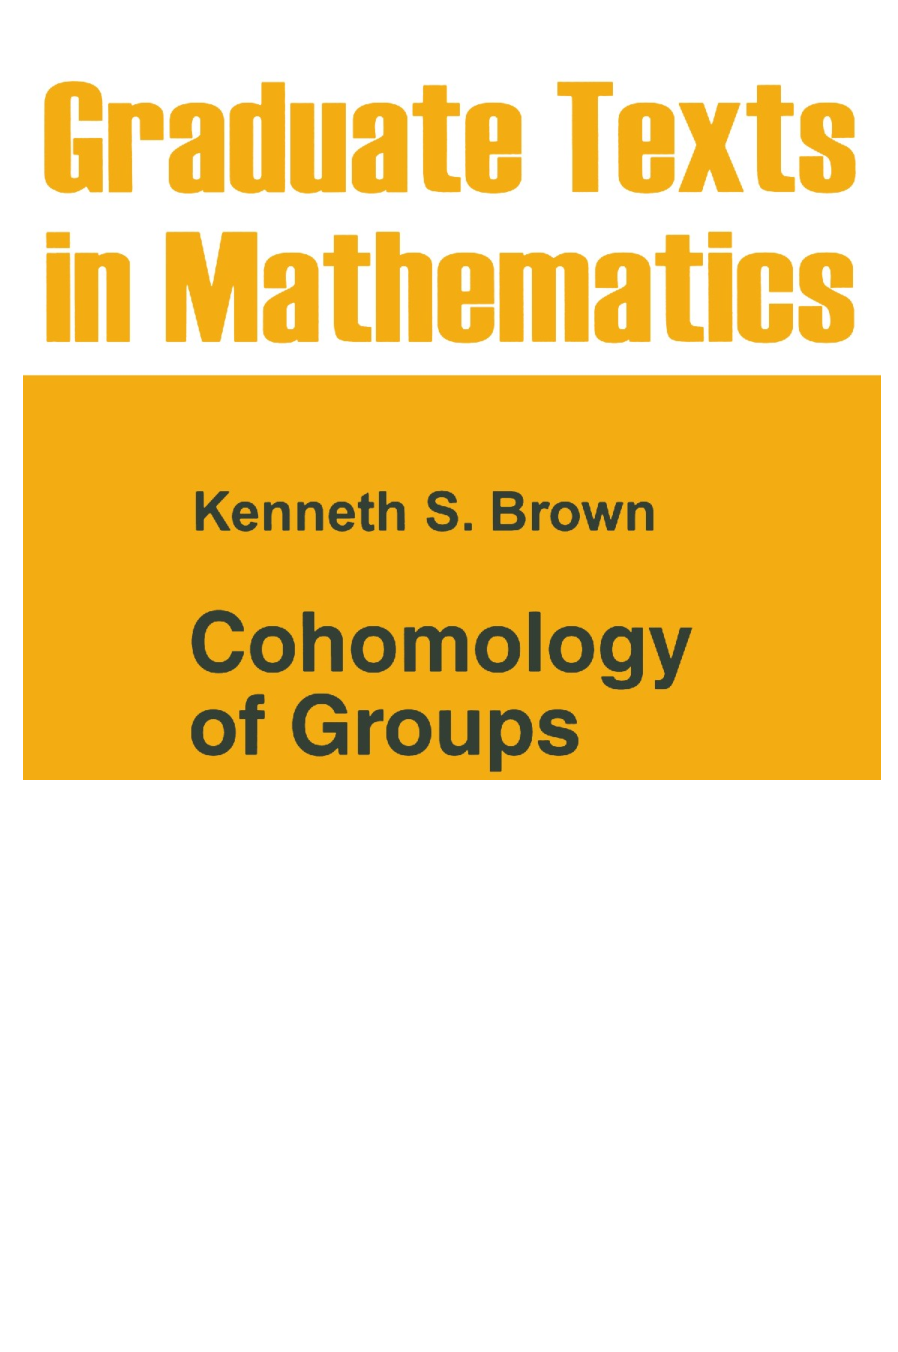
\includegraphics[height=2cm]{../spspt/brown_book}
	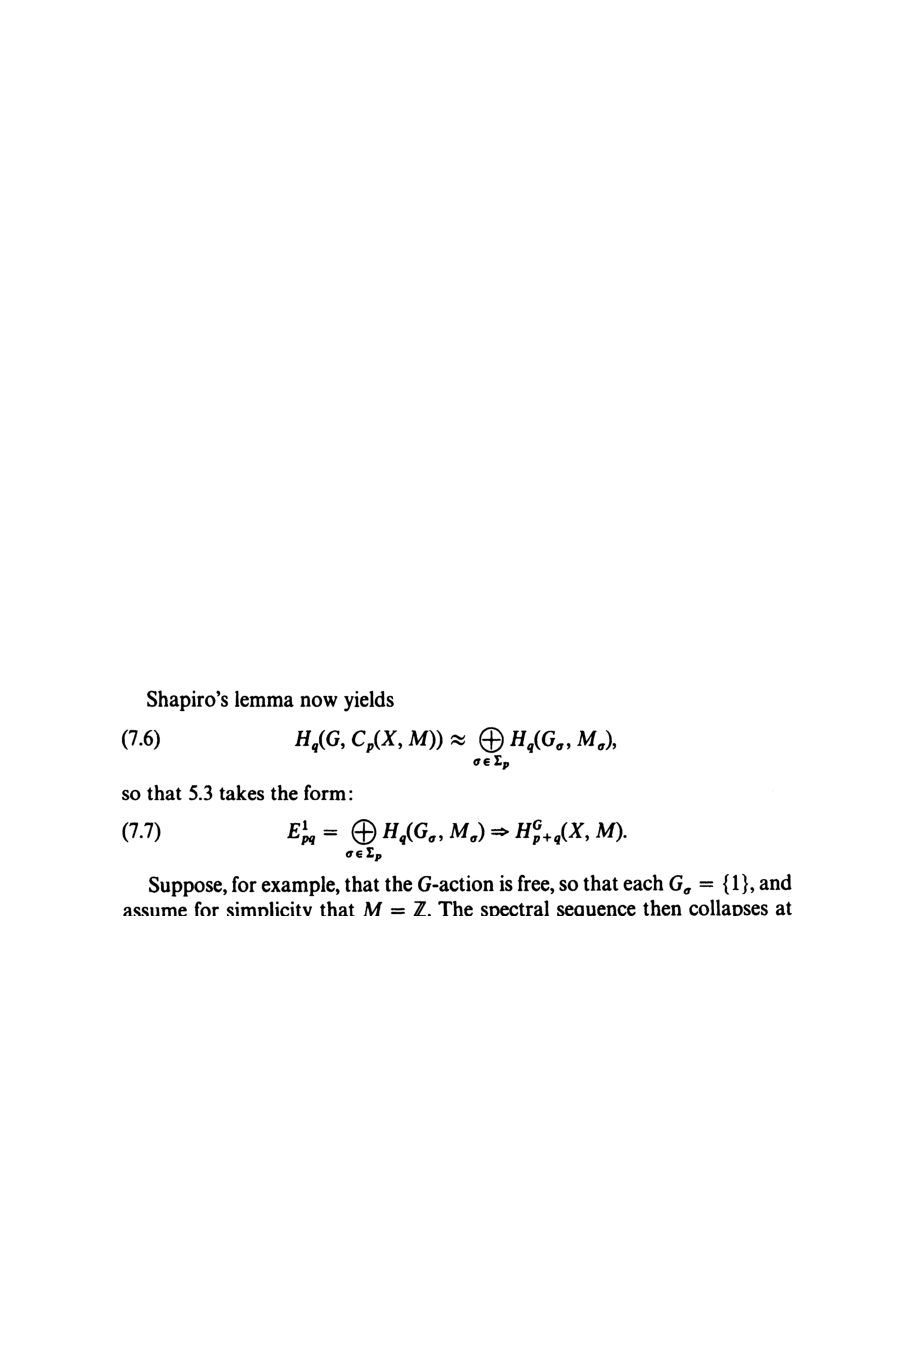
\includegraphics[height=2cm]{../spspt/brown_ss}
\end{center}
\end{frame}

\begin{frame}
\frametitle{An example of a nontrivial building block}
Consider $G=SG\times\mathbb Z_2$, $SG=P4_22_12$ (\#94 space group).
\begin{center}
\includegraphics[height=4cm]{../spspt/blocks}
\end{center}
Each colored 2-cell is decorated with a Levin-Gu or CZX state protected by the onsite $\mathbb Z_2$.

\emph{\small Adapted from Z Song, Y Huang, YQ, C Fang and M Hermele, Sci Adv 2019.}
\end{frame}

\begin{frame}
	\frametitle{Results for all 230 space groups}
	\begin{columns}
		\column{.6\textwidth}
		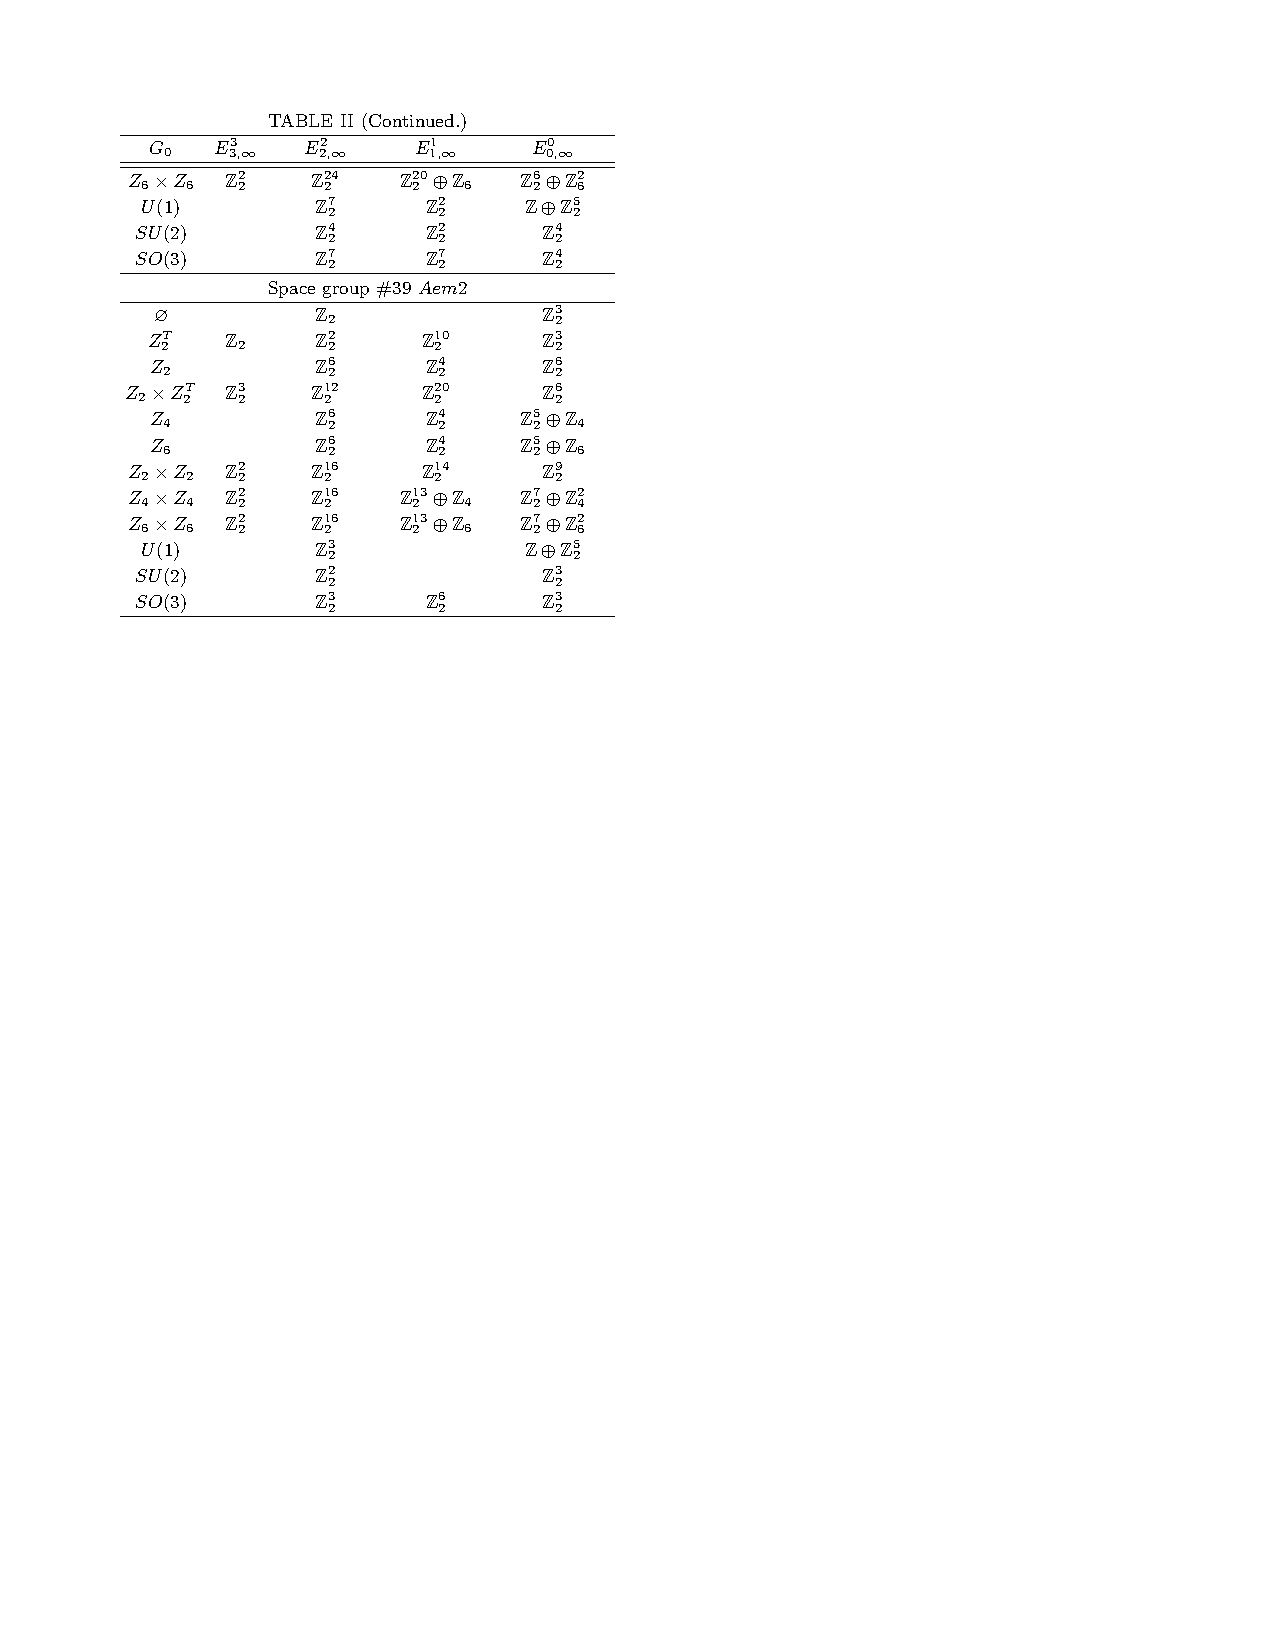
\includegraphics[height=8cm]{../spspt/bigtable}
		\column{.4\textwidth}
		\begin{itemize}
			\item Classifications computed for all 230 space groups, paired with selected $G_0$.
			\item Results computed by a fully automated python code.
		\end{itemize}
	\end{columns}
\end{frame}

\begin{frame}
\frametitle{An example of 2nd order computation}
\emph{\small Adapted from Xu Yang, Shenghan Jiang, Ashvin Vishwanath and Ying Ran, Ann Phys \textbf{413}, 168060 (2019)..}
\begin{itemize}
	\item Consider a magnetic translation symmetry $T_xT_yT_x^{-1}T_y^{-1} = X$, and $G_0=\mathbb Z_2^X\times\mathbb Z_2^T$.
	\item $H^3[G_0,\uone_T]=\mathbb Z_2\oplus\mathbb Z_2$: the one protected by both $\mathbb Z_2^X$ and $\mathbb Z_2^T$ is \alert{not compatible} with the magnetic translation symmetry.
	\item Try to decorate $\omega\in H^3[G_0,\uone_T]$ to all 2-cells: the 1-cells can be gapped out, but the 0-cells \alert{cannot}.
	\item There must be a $T^2=-1$ Kramers doublet at each 0-cell.
\end{itemize}
\begin{center}
\begin{tikzpicture}
\draw (-1.2,0)--(1.2,0);
\draw (-1.2,1)--(1.2,1);
\draw (-1.2,-1)--(1.2,-1);
\draw (-1,-1.2)--(-1,1.2);
\draw (0,-1.2)--(0,1.2);
\draw (1,-1.2)--(1,1.2);
\fill [red] (-1,-1) circle (2pt);
\fill [red] (-1,0) circle (2pt);
\fill [red] (-1,1) circle (2pt);
\fill [red] (0,-1) circle (2pt);
\fill [red] (0,0) circle (2pt);
\fill [red] (0,1) circle (2pt);
\fill [red] (1,-1) circle (2pt);
\fill [red] (1,0) circle (2pt);
\fill [red] (1,1) circle (2pt);
\end{tikzpicture}
\end{center}
\end{frame}

\section{Computing interacting-fermion SPT classification}

\begin{frame}
	\frametitle{Fermionic SPT: a generalized cohomology theory}
	\begin{itemize}
        \item An Atiyah–Hirzebruch Spectral Sequence: an fSPT state is specified by several layers.
          \[E^{pq}_2=H^p[G_b, H^q(\text{pt}, ??)]]\Rightarrow H^{p+q}(BG_b, ??).\]
        \item Example: 2D fSPT,
          \begin{enumerate}
          \item $n_1\in H^1[G, \mathbb Z_2]$: Majorana-chain decoration.
          \item $n_2\in C^2[G, \mathbb Z_2]$: Complex-fermion decoration.
          \item $\nu_3\in C^3[G, \uone]$: Bosonic phase factor.
          \item A real-space construction: Q-R Wang and Z-C Gu, PRX 2020.
          \end{enumerate}
	\end{itemize}
\end{frame}

\begin{frame}
	\frametitle{Fermionic SPT: a generalized cohomology theory}
	\begin{itemize}
		\item Obstruction functions: higher-page derivatives of the spectral sequence.
		\item Example: checking if $n_1\in H^1[G, \mathbb Z_2]$ is obstructed?
		\begin{enumerate}
			\item Check $\mathcal O_3[n_1] = \omega_2\cup n_1 + s_1\cup n_1\cup n_1$ vanishes.
			\item Find $n_2$ such that $dn_2 = \mathcal O_3[n1]$.
			\item Check $\mathcal O_4[n_2]$ vanishes.
			\begin{align*}\mathcal O_4(01234) = \frac12\big[\omega_2\cup n_2 + n_2\cup n_2 + n_2 \cup_1 dn_2 + \omega_2(013)dn_2(1234)\\ + dn_2(0124)dn_2(0234)\big]
			-\frac14\big\{dn_2(0123)[1-dn_2(0124)]\text{ (mod 2)}\big\}.
		\end{align*}
		\end{enumerate}
		This defines a map between cohomology classes
		$n_1\mapsto \mathcal O_4$.
		\item In theory, this is the end of the story. But in practice...
	\end{itemize}
\end{frame}

\begin{frame}
	\frametitle{Computational cost}
	\begin{itemize}
		\item Key step: solving the cocycle/coboundary equation; finding $\ker d^n$ and $\img d^{n-1}$.
		\item ``Diagonalizing'' the coboundary matrix $d^n$: Smith Normal Form.
		\item $d^n$ acts on $\alpha(g_1,\ldots,g_n)$: $(|G|-1)^n$-dimension.
		\item Complexity = $O(N^3)$, $N = (|G|-1)^n$.
		\item Quite expensive for large $G$ ($|G| > 16$); infinite for $|G|=\infty$ (wallpaper and space groups).
	\end{itemize}
	\begin{block}{Can we do better?}
		\begin{itemize}
			\item For bSPTs: $H^n[G,\uone]$ can be computed using simpler $BG$.
			\item What about fSPTs and other cases w/ complicated maps b/w cohomology groups?
		\end{itemize}
	\end{block}
\end{frame}

\begin{frame}
	\frametitle{Other similar tasks}
	\begin{itemize}
		\item Symmetry-Enriched Topological (SET) states: ($\mathcal C^\times_G$)\\
		Maissam Barkeshli and Meng Cheng, arXiv:1906.10691.

		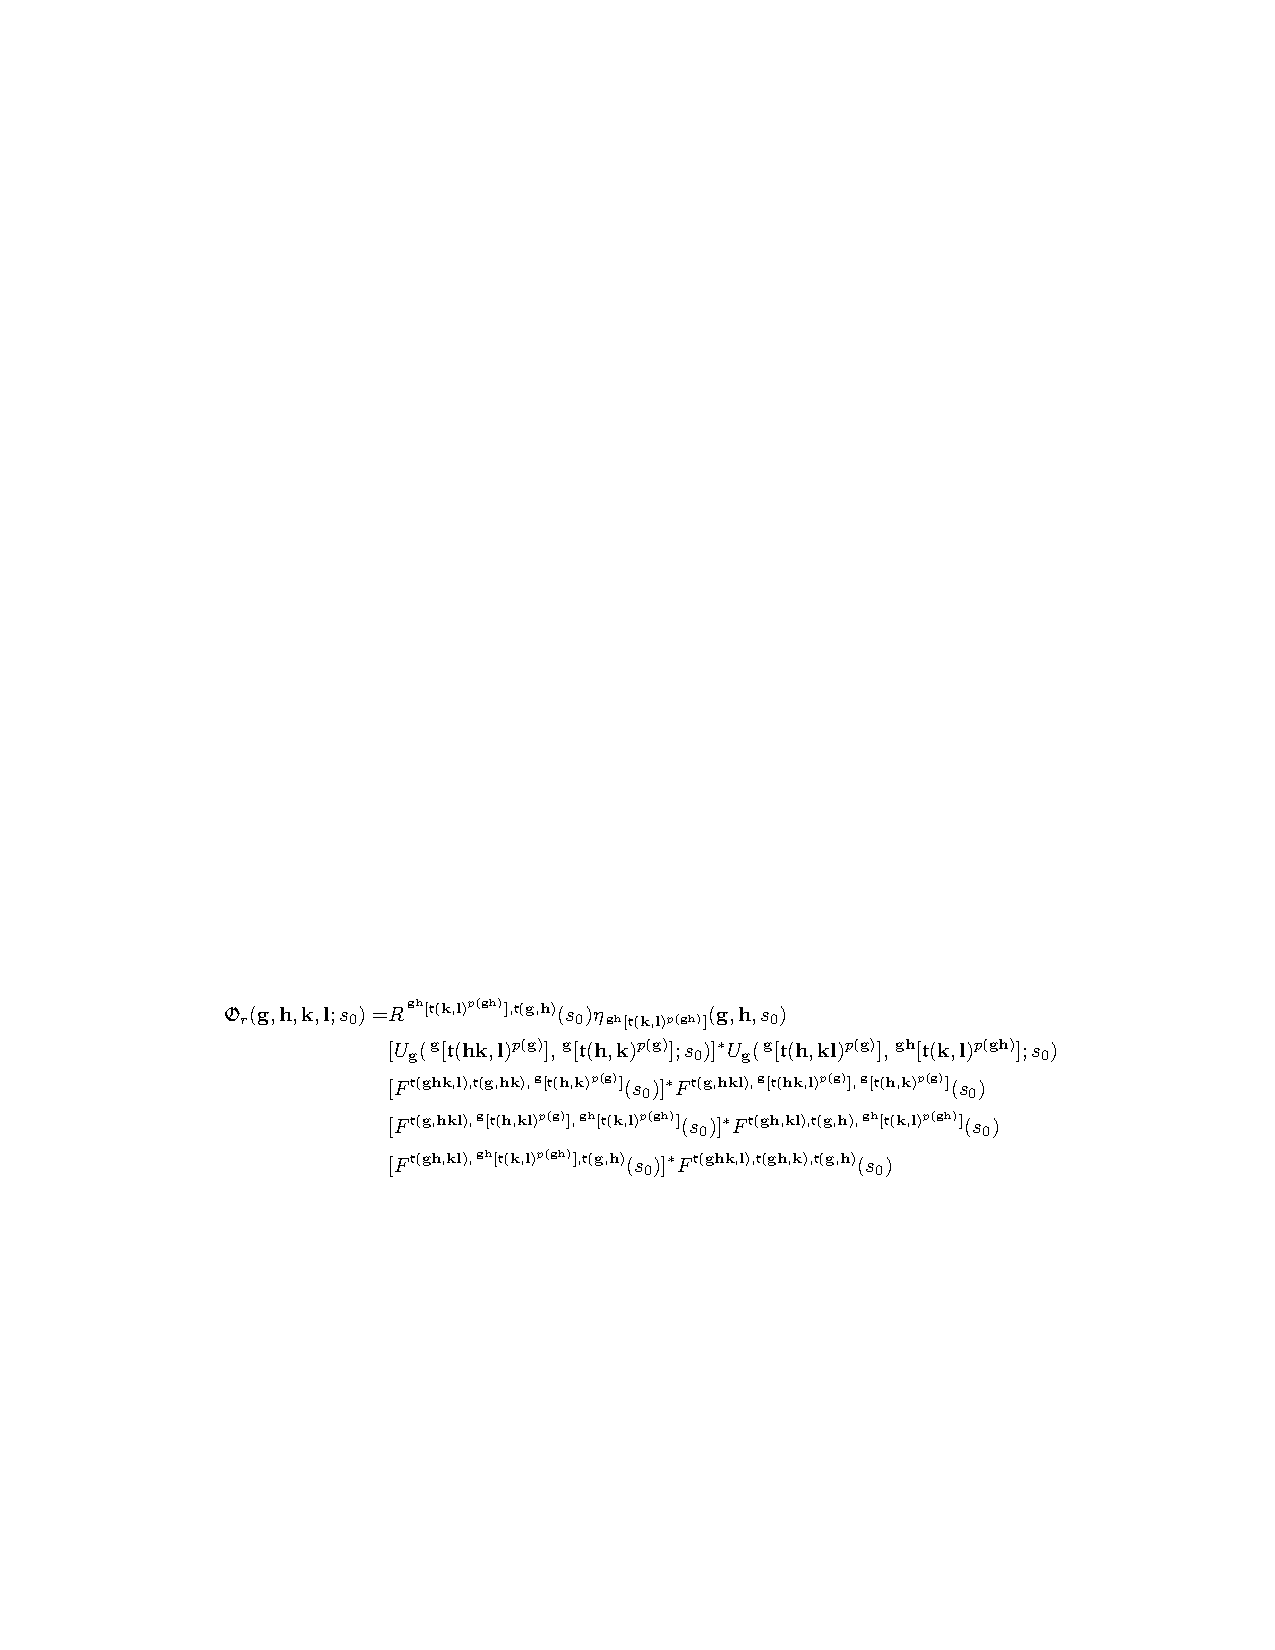
\includegraphics[scale=.8]{../chainmap/relanomaly_eq}
		\item 3D U(1) spin liquids:\\
		Shang-Qiang Ning, Liujun Zou and Meng Cheng, arXiv:1905.03276.

		
\includegraphics[scale=.8]{../chainmap/u1sl_eq}
	\end{itemize}
\end{frame}

\begin{frame}
	\frametitle{Our goal}
	\begin{itemize}
		\item Our goal: develop an algorithm to accelerate the computation of cohomology groups of $G$ and mapping between cohomology groups.
		\item Why we want a faster computation?
		\begin{enumerate}
			\item fSPT: Some nontrivial decorations and decorations only appear for complicated $G$.
			\item Realistic system: crystalline-symmetry groups $|G|=\infty$.
		\end{enumerate}
		\item We want to develop an easy-to-use software package for computing fSPT and SET classifications.
		\item A live demo of what we have now...
	\end{itemize}
\end{frame}

\begin{frame}
	\frametitle{A standard and a simplified construction of $BG$}
	\begin{enumerate}
		\item Standard construction: $BG$ as a simplicial complex.
		\begin{itemize}
			\item All cells are simplices, $[g_1|g_2|\cdots|g_n]$.
			\item Uniform boundary operations:
			$\partial[g_1|g_2]=g_1[g_2]-[g_1g_2]+[g_1]$, ...
			\item Requires many cells.
		\end{itemize}
		\item Simplified construction: $BG$ as a CW-complex.
		\begin{itemize}
			\item Cells have arbitrary shapes.
			\item Arbitrary boundary operations.
			\item Can have very few cells.
		\end{itemize}
	\end{enumerate}
	\begin{center}
		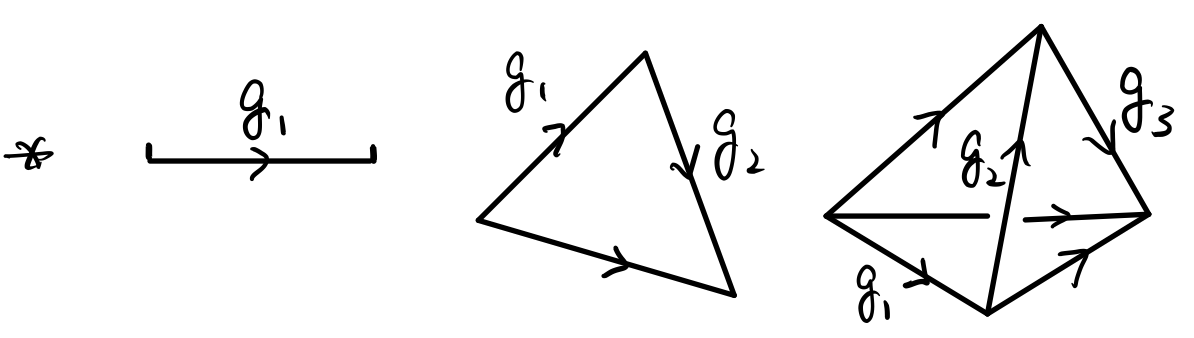
\includegraphics[width=10cm]{../chainmap/bg-std}~~~~
		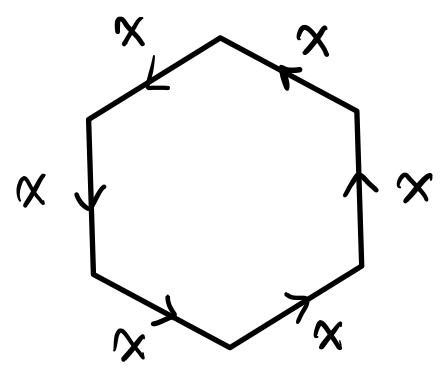
\includegraphics[height=3cm]{../chainmap/z6-1}
	\end{center}
\end{frame}

\begin{frame}
	\frametitle{Computing the group cohomology using $BG$}
	\begin{itemize}
		\item $H^D[G, \uone] = H^D[BG, \uone]$: need to compute the cohomology group of $BG$.
		\item The coboundary operator $d^n$ is a matrix of size $|X_n(BG)|\times |X_{n+1}(BG)|$.
		\item Complexity: $|X_n(BG)|^3$.
		\item It is much easier to compute for the simplified $BG$.
		\item $BG$ is actually simple when $G$ is infinite but torsion-free:
		$B\mathbb Z=S^1$, $B\mathbb Z^2=T^2$, etc.
	\end{itemize}
\end{frame}

\begin{frame}
	\frametitle{How to compute cohomology operations}
	\begin{itemize}
		\item Consider $f: H^p[G,\uone]\rightarrow H^{p'}[G, \uone]$.
		\item In general, we do not know how to derive the formula for a simplified $BG$.
		\item Map to/from the standard $BG$: a dictionary translating b/w two types of cohomology classes.
		\[H^p[BG_1,\uone]\simeq H^p[BG_2,\uone].\]
		\item Algorithm:
		\begin{enumerate}
			\item Consider $\alpha$ on simplified $BG$.
			\item Convert to $\bar\alpha$ on standard $BG$.
			\item Compute $\bar\beta = f(\bar\alpha)$ using existing formula.
			\item Map $\bar\beta$ to $\alpha$ on the simplified $BG$.
			\item Check whether $\alpha$ is trivial.
		\end{enumerate}
	\end{itemize}
\end{frame}

\begin{frame}
	\frametitle{Algebraic version: resolution}
	\begin{itemize}
		\item We do not need that much of geometric information of $BG$.
		\item Chain complex (augmented) of $EG$ ($EG/G=BG$)
                {\small\[\cdots\rightarrow C_k(EG)\xrightarrow{\partial_k}
		C_{k-1}(EG)\rightarrow\cdots\rightarrow
		C_1(EG)\xrightarrow{\partial_1}
		C_0(EG)\xrightarrow{\epsilon}\mathbb Z\rightarrow0.\]}
		\item Free resolution:
		{\small\[\cdots\rightarrow F_k\xrightarrow{\partial_k}
		F_{k-1}\rightarrow\cdots\rightarrow
		F_1\xrightarrow{\partial_1}
		F_0\xrightarrow{\epsilon}\mathbb Z\rightarrow0.\]}
		\item Forms a long exact sequence of free $\mathbb ZG$-modules.
		\item Cochain: $C^k=\hhom_G[F_k, \uone]$
		\item Coboundary: $d^n:C^n\rightarrow C^{n+1}$, $d^n\alpha(x) = \alpha(\partial x)$.
		\item Cohomology group: $H^n[G, \uone]=\frac{\ker d^n}{\img d^{n-1}}$.
	\end{itemize}
\end{frame}

\begin{frame}
	\frametitle{Example: bar resolution and inhomogeneous cocycle}
	\begin{itemize}
		\item Consider the (normalized) bar resolution:
		$F_n$ is generated by $[g_1|\cdots|g_n]$.
		\item Boundary map:
		\[\partial[g_1|\cdots|g_n]=g_1[g_2|\cdots|g_n]
		-[g_1g_2|\cdots|g_n]+[g_1|g_2g_3|\cdots|g_n]-\cdots.\]
		\item This gives the inhomogeneous cocycle:
		$\alpha([g_1|\cdots|g_n])=\alpha(g_1,\ldots,g_n)$.
		\item This corresponds to the standard construction of $BG$.
	\end{itemize}
\begin{center}
	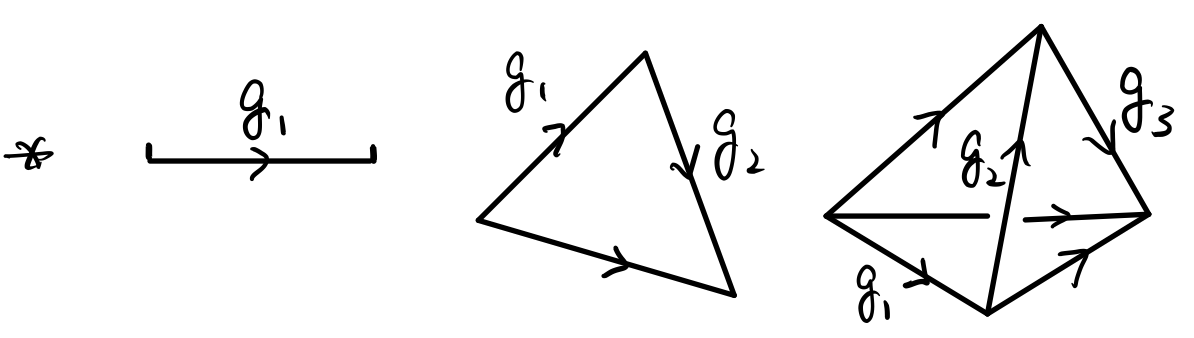
\includegraphics[width=10cm]{../chainmap/bg-std}
\end{center}
\end{frame}

\begin{frame}[fragile]
	\frametitle{Chain map between two resolutions}
	\begin{itemize}
		\item Consider two resolutions: simplified resolution $F$ and bar resolution $F'$.
		\item We can construct chain maps $f:F\rightarrow F'$ and $g:F'\rightarrow F$, such that
		{\small\[\begin{tikzcd}
		\cdots\arrow[r,"\partial_{k+1}"]&
		F_k\arrow[r,"\partial_k"]\arrow[d,"f_k"]&
		F_{k-1}\arrow[r,"\partial_{k-1}"]\arrow[d,"f_{k-1}"]&
		\cdots\arrow[r,"\partial_2"]&
		F_1\arrow[r,"\partial_1"]\arrow[d,"f_1"]&
		F_0\arrow[r,"\epsilon"]\arrow[d,"f_0"]&
		\mathbb Z\arrow[d,"\id"]\\
		\cdots\arrow[r,"\partial_{k+1}'"]&
		F_k'\arrow[r,"\partial_k'"]&
		F_{k-1}'\arrow[r,"\partial_{k-1}"]&
		\cdots\arrow[r,"\partial_2'"]&
		F_1'\arrow[r,"\partial_1'"]&
		F_0'\arrow[r,"\epsilon'"]&
		\mathbb Z
		\end{tikzcd}\]
		commutes.
		\item $f^\ast$ and $g^\ast$ maps between two types of cocycles:
		\[f^\ast:C^{n\prime} = \hhom_G[F^\prime_n,\uone]\rightarrow C^n=\hhom_G[F_n,\uone]:
		f^\ast\alpha(x)=\alpha(f(x)).\]}
	\end{itemize}
\end{frame}

\begin{frame}[fragile]
	\frametitle{Use chain maps to compute comohomogy operations}
	\begin{itemize}
		\item We want to compute a map $C^m\rightarrow C^n$.
		\item We only know the formula $C^{m\prime}\rightarrow C^{n\prime}$.
		\item Use $f^\ast$ and $g^\ast$:
	\end{itemize}
	\[\begin{tikzcd}
		C^m\arrow[r,dashrightarrow]\arrow[d,"g^\ast"] & C^n\\
		C^{m\prime}\arrow[r] & C^{n\prime}\arrow[u,"f^\ast"]
	\end{tikzcd}\quad\quad\quad
	\begin{tikzcd}
		\alpha\arrow[d,"g^\ast",mapsto] & \beta\\
		\alpha'\arrow[r,mapsto] & \beta'\arrow[u,"f^\ast",mapsto]
	\end{tikzcd}
	\]
\end{frame}

\begin{frame}[fragile]
	\frametitle{Contracting homotopy of a resolution}
	\begin{itemize}
		\item Since $F$ is a long exact sequence, we can construct a contracting homotopy: $\id:F\rightarrow F$ is homotopic to $0:F\rightarrow F$.
		\item A contracting homotopy $s_k: F_k\rightarrow F_{k+1}$
		\[
		\begin{tikzcd}
		F_{k+1} \arrow[r,"\partial_{k+1}"]
		&F_k\arrow[r,"\partial_k"]
		\arrow[d,"\id"]
		\arrow[ld,"s_k"]&
		F_{k-1}\arrow[ld,"s_{k-1}"]\\
		F_{k+1} \arrow[r,"\partial_{k+1}"]& F_k\arrow[r,"\partial_k"]&
		F_{k-1}
		\end{tikzcd}
		\]
		such that $\partial_{k+1}s_k + s_{k-1}\partial_k = \id$.
		\item $s$ can be used to compute the preimage of $\partial$: If $\partial x=0$, then $\partial s(x) = x$.
		\item For the bar resolution, $s(g_0[g_1|\cdots|g_n])
		=[g_0|g_1|\cdots|g_n]$.
		\item In practice, $s$ is constructed along with the simplified resolution $F$.
	\end{itemize}
\end{frame}

\begin{frame}[fragile]
	\frametitle{Constructing the chain map}
	\begin{itemize}
		\item We construct the chain map recursively,
		\[\begin{tikzcd}
		\cdots\arrow[r,"\partial_5"]&
		F_4\arrow[r,"\partial_4"]\only<6->{\arrow[d,"f_4"]}&
		F_3\arrow[r,"\partial_3"]\only<5->{\arrow[d,"f_3"]}&
		F_2\arrow[r,"\partial_2"]\only<4->{\arrow[d,"f_2"]}&
		F_1\arrow[r,"\partial_1"]\only<3->{\arrow[d,"f_1"]}&
		F_0\arrow[r,"\epsilon"]\only<2->{\arrow[d,"f_0"]}&
		\mathbb Z\arrow[d,"\id"]\\
		\cdots\arrow[r,"\partial_5'"]&
		F_4'\arrow[r,"\partial_4'"]&
		F_3'\arrow[r,"\partial_3"]&
		F_2'\arrow[r,"\partial_2'"]&
		F_1'\arrow[r,"\partial_1'"]&
		F_0'\arrow[r,"\epsilon'"]&
		\mathbb Z
		\end{tikzcd}\]
		\item In each step:
		\begin{columns}
			\column{.3\columnwidth}
			\[\begin{tikzcd}
			F_{n+1}\arrow[r,"\partial"]\arrow[d,"f_{n+1}",dashrightarrow]
			&F_n\arrow[d,"f_n"]\\
			F_{n+1}'\arrow[r,"\partial'"]&F_n'
			\end{tikzcd}\]
			\column{.7\columnwidth}
			\begin{enumerate}
				\item Choose a $\mathbb ZG$ basis $e^{n+1}_i$.
				$\partial'f_{n+1}(e^{n+1}_i) = f_n(\partial e^{n+1}_i).$
				\item Let $f_{n+1}(e^{n+1}_i)=s'(f_n(\partial e^{n+1}_i))$.
				\item Extend $f_{n+1}$ linearly to $F_{n+1}$.
			\end{enumerate}
		\end{columns}
	\end{itemize}
\end{frame}

\begin{frame}
	\frametitle{Constructing a simplified resolution}
	\begin{enumerate}
		\item Using the HAP package in the GAP software: \url{www.gap-system.org}.\\
		G. Ellis, J. Symb. Comput. \textbf{38}, 1077 (2004).
		\item Simple resolution for Abelian groups $\mathbb Z_n$.
		\item Wall's construction: CTC Wall, Math. Proc. Cam. Phil. Soc. \textbf{57}, 251 (1961).\\
		Given a group extension $1\rightarrow N\rightarrow G\rightarrow Q\rightarrow 1$, and resolutions of $N$ and $Q$: $F_N$ and $F_Q$, a resolution of $G$ can be constructed as a ``perturbation'' of $F_N\otimes F_Q$.
		\item Use Wall's construction, we can compute a simplified resolution for $G$ if $G$ is written as a series of group extensions:
		\[G=G_1\supset G_2\supset\cdots\supset G_n=\mathbb Z_1\]
		such that $G_i/G_{i+1}=\mathbb Z_{m_i}$ or $\mathbb Z$.\\
		This method works for all wallpaper and space groups.
	\end{enumerate}
\end{frame}

\begin{frame}
	\frametitle{Lazy evaluation}
	\begin{itemize}
		\item Lasy evaluation: compute $\alpha(g_1,\ldots,g_n)$ only when it is needed.
		\item Allows computation for $|G|=\infty$.
		\item Scheme:
		\[\alpha(e^4_i)\Rightarrow \alpha(g_1,g_2,g_3,g_4)
		\Rightarrow \frac12\beta(g_1,g_2)\beta(g_3,g_4)\Rightarrow \beta(e^2_j).\]
	\end{itemize}
	\begin{center}
		
\includegraphics[height=3cm]{../chainmap/geyou}
	\end{center}
\end{frame}

\begin{frame}[fragile]
	\frametitle{A subtlety: how to solve a cocycle equation}
	\begin{itemize}
		\item Task: given inhomogeneous cocycle $\beta'$, find solution $\alpha'$ such that $d\alpha'=\beta'$
		\item Use $f:F\rightarrow F'$ and $g:F'\rightarrow F$.
		\item Naively: $\beta'\Rightarrow\beta = f^\ast\beta'\Rightarrow d\alpha = \beta\Rightarrow\alpha'=g^\ast\alpha$.
		\item However, this does not work because $f\circ g: F'\rightarrow F\rightarrow F'$ is not id.
		\item $f\circ g$ is homotopic to $\id_{F'}$: construct a homotopy equivalence $h: f\circ g\sim \id_{F'}$.
		\[\alpha' = g^\ast\alpha \alert{- h^\ast\beta'}.\]
	\end{itemize}
	\begin{block}{Homotopy equivalence}
		\begin{columns}
			\column{.4\columnwidth}
			\[\begin{tikzcd}
			    F'_{k+1}\arrow[r,"\partial_{k+1}"]\arrow[d]&
			    F'_k\arrow[r, "\partial_k"]
			    \arrow[d, ""]
			    \arrow[ld, "h_k"]&
			    F'_{k-1}\arrow[ld, "h_{k-1}"]\arrow[d]\\
			    F_{k+1}\arrow[r,"\partial_{k+1}"]&
			    F'_k\arrow[r, "\partial_k"]&
			    F'_{k-1}
			  \end{tikzcd}\]
			\column{.6\columnwidth}
			\begin{itemize}
				\item $h$ is a deg-1 map: $h_k:F'_k\rightarrow F'_{k+1}$
				\item s.t. $\partial_{k+1}h_k + h_{k-1}\partial_k
				=f_kg_k-\id_{F'_k}$.
				\item Can also be constructed recursively.
			\end{itemize}
		\end{columns}
	\end{block}
\end{frame}

\begin{frame}
	\frametitle{Similar techniques}
	\begin{itemize}
		\item The chain maps to/from bar resolution is already implemented in HAP, which is used to compute the homology groups of the classifying space of 2-groups.\\
		Graham Ellis and Le Van Luyen, J. Symb. Comput. \textbf{47}, 1309 (2012).
		\item We implemented our own version of the chain maps, which are faster than the HAP version.
		\item Applied to the task of computing fSPT and SET classifications.
	\end{itemize}
\end{frame}

\begin{frame}[fragile]
	\frametitle{GAP, HAP and group cohomology}
	\begin{itemize}
		\item bSPT: $H^D[G,\uone]$ can be computed directly using HAP in GAP.
		\item $H^D[G,\uone]$ ``='' $H^{D+1}[G,\mathbb Z]$. \emph{See X-G Wen, PRB \textbf{91}, 205101 (2015)}
	\end{itemize}
	\begin{columns}
		\column{.5\columnwidth}
	\begin{lstlisting}[basicstyle=\footnotesize]
gap> LoadPackage("HAP");
gap> G := CyclicGroup(4);
pc group of size 4 with 2 generators>
gap> GroupCohomology(G, 2);
[ 4 ]
gap> GroupCohomology(G, 3);
[  ]
gap> GroupCohomology(G, 4);
[ 4 ]
gap> GroupCohomology(G, 5);
[  ]
\end{lstlisting}
	\column{.5\columnwidth}
	\[H^{2n+1}[\mathbb Z_4,\uone] = \mathbb Z_4\]
	\[H^{2n}[\mathbb Z_4,\uone] = \mathbb Z_1\]
	\end{columns}
\end{frame}

\begin{frame}[fragile]
	\frametitle{Implimenting chain maps in GAP}
	\begin{itemize}
		\item We are working on a GAP package to impliment the chain maps and to compute fSPT classifications.
		\item User only need to input the mappingin terms of inhomogeneous cocycles.
		\item The package automatically computes the mapping using the simplified resolution.
	\end{itemize}
\begin{lstlisting}[basicstyle=\footnotesize,morekeywords={function,return,local,if,fi,then,end},showspaces=false,showtabs=false, keywordstyle=\color{blue}]
SptSetInstallCoboundary(ss, 2, 2, 1,
function(n2, dn2)
  return function(g1, g2, g3, g4)
    local val;
    val := 1/2 * (n2(g1, g2) * n2(g3, g4) mod 2);
    if dn2 <> ZeroCocycle@ then
      val := val + 1/2 * ((n2(g1*g2*g3, g4) * dn2(g1, g2, g3)
        + n2(g1, g2*g3*g4) * dn2(g2, g3, g4)) mod 2);
      val := val + 1/2 * (dn2(g1, g2, g3*g4) * dn2(g1*g2, g3, g4) mod 2);
      val := val - 1/4 * (dn2(g1, g2, g3) * (1 - dn2(g1, g2, g3*g4)) mod 2);
    fi;
    return val;
  end;
end);
\end{lstlisting}
\end{frame}

\begin{frame}[fragile]
	\frametitle{Example: computing fSPT}
	Consider 2D fSPT, $G=\mathbb Z_4$:
\begin{lstlisting}[basicstyle=\footnotesize]
gap> LoadPackage("SptSet");;
gap> G := CyclicGroup(4);;
gap> R := ResolutionFiniteGroup(G, 6);;
gap> utAct := SptSetTrivialGroupAction(G);;
gap> ss := FermionEZSPTSpecSeq(R, utAct);;
gap> FermionSPTLayers(ss, 2);
[ <ZL-Module with torsions [ 2 ]>, <ZL-Module with torsions [ 2 ]>,
  <ZL-Module with torsions [ 4 ]> ]
gap> z2tAct := GroupHomomorphismByImagesNC(G, GL(1, Integers),
>   GeneratorsOfGroup(G), [ [[-1]], [[1]] ]);;
gap> ss := FermionEZSPTSpecSeq(R, z2tAct);;
gap> FermionSPTLayers(ss, 2);
[ <ZL-Module with torsions [ 2 ]>, <ZL-Module []>, <ZL-Module []> ]
\end{lstlisting}

Example: compute fSPT for 2D wallpaper groups.
\end{frame}

\begin{frame}
	\frametitle{Summary}
	\begin{itemize}
		\item Use a simplified free resolution to accelerate computation of group cohomology.
		\item Use chain maps between resolutions to compute maps between cohomology groups.
		\item We are working on a GAP package SptSet.
		\item Takes 5min to compute 2D fSPTs for all 17 wallpaper groups.
		\item Email me at \url{qiyang@fudan.edu.cn} for early access.
		\item We also have a program written in python: faster but much harder to use.
		\item Will add more functions (fSPT with nontrivial group extension, group structure, ...), tweak the performence, and publish.
	\end{itemize}
\end{frame}

\section{Outlooks}

\begin{frame}
  \frametitle{Summary: the status of the field now}
  \begin{itemize}
  \item[\ding{51}] Bosonic SPT states: both onsite and space-group symmetries.
  \item[\ding{51}] Free-fermion SPT states: onsite symmetries. (10-fold way).
  \item[?] Free-fermion SPT states: crystalline symmetries.
  \item[?] Interacting-fermion SPT states: onsite symmetries and crystalline symmetries.
  \item[\ding{55}] Realization in materials.
  \end{itemize}
\end{frame}

\begin{frame}
  \frametitle{Future directions}
  \begin{itemize}
  \item Interacting-fermion SPT classification: the most general formula and fast computation.
  \item Crystalline-SPT states: real-space construction (fermionic cases) and high-order corner states.
  \item Measuring bulk SPT invariants: measuring partition functions with nontrivial space-time topology and symmetry fluxes; high-order correlation functions; ...\\
    \emph{\small}
  \item Phase transitions between SPT phases.\\
    \emph{\small L Tsui, H-C Jiang, Y-M Lu and D-H Lee, Nuclear Phys B 2015}
  \end{itemize}
\end{frame}

\end{document}
